% Created by tikzDevice version 0.7.0 on 2014-06-29 19:47:51
% !TEX encoding = UTF-8 Unicode
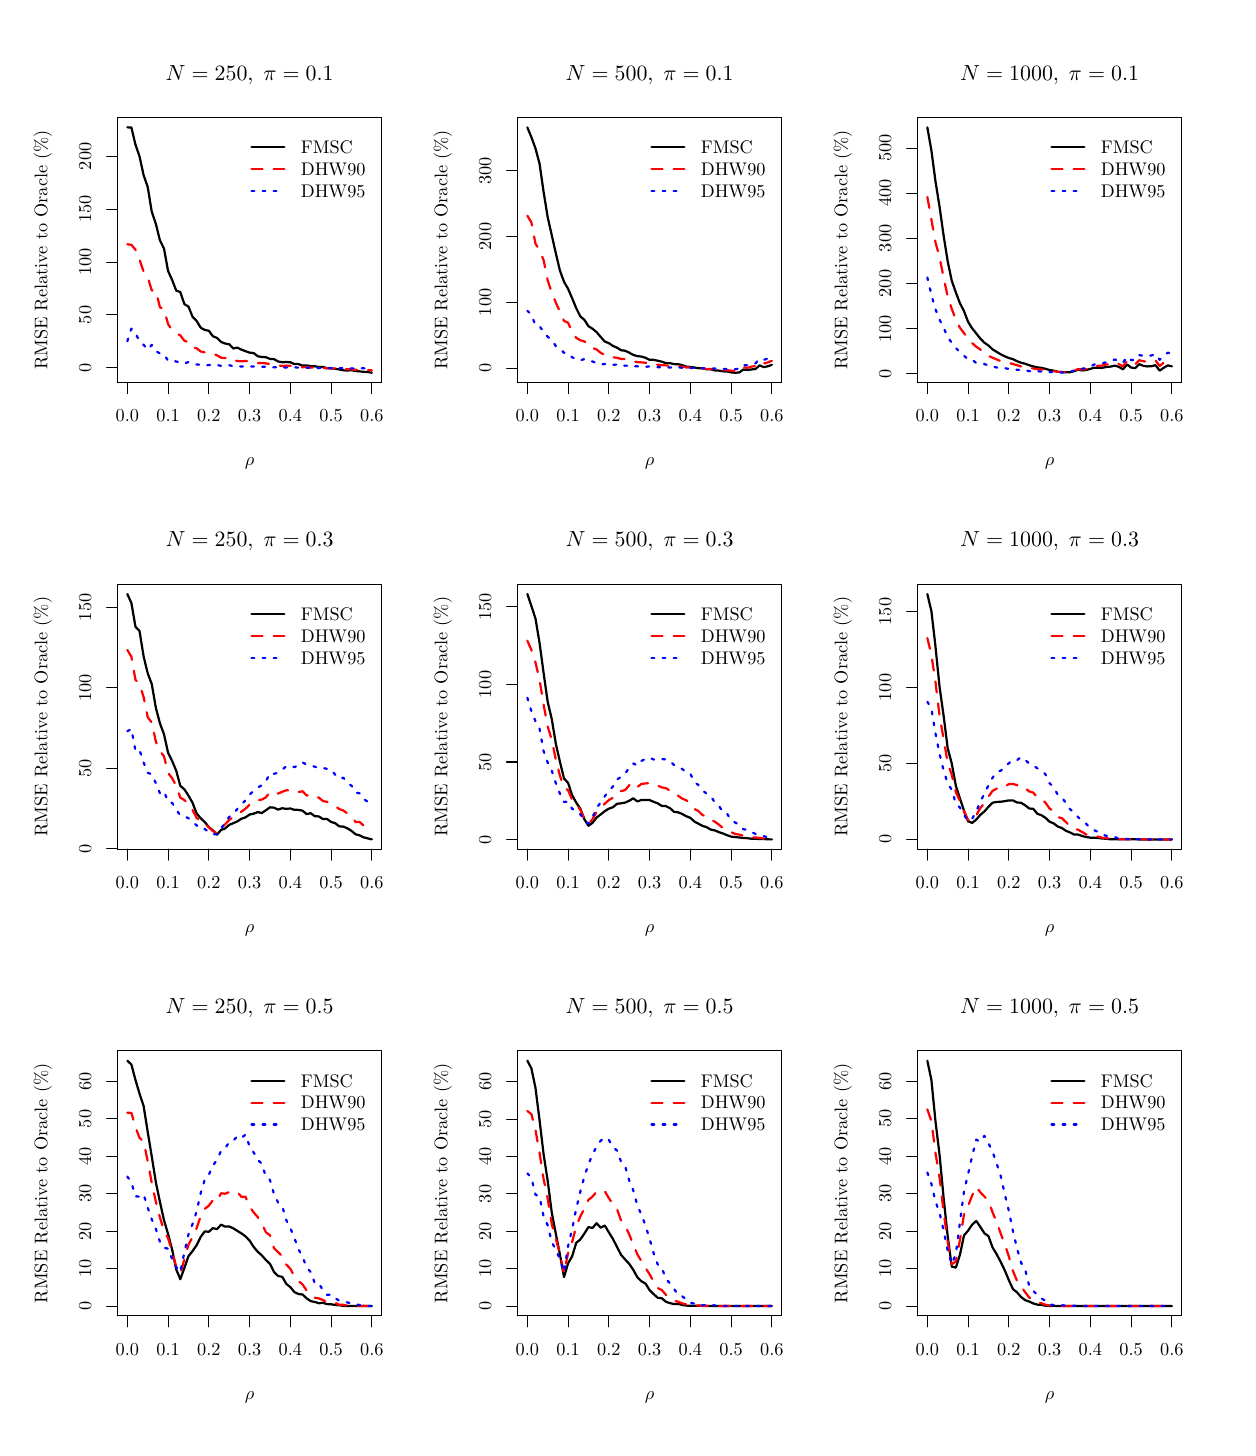
\begin{tikzpicture}[x=1pt,y=1pt]
\definecolor[named]{fillColor}{rgb}{1.00,1.00,1.00}
\path[use as bounding box,fill=fillColor,fill opacity=0.00] (0,0) rectangle (433.62,505.89);
\begin{scope}
\path[clip] ( 32.47,377.65) rectangle (127.91,473.42);
\definecolor[named]{drawColor}{rgb}{0.00,0.00,0.00}

\path[draw=drawColor,line width= 0.8pt,line join=round,line cap=round] ( 36.01,469.87) --
	( 37.48,469.80) --
	( 38.95,463.61) --
	( 40.42,459.37) --
	( 41.90,452.57) --
	( 43.37,448.33) --
	( 44.84,439.35) --
	( 46.32,434.95) --
	( 47.79,429.04) --
	( 49.26,426.07) --
	( 50.73,417.97) --
	( 52.21,414.71) --
	( 53.68,410.87) --
	( 55.15,410.37) --
	( 56.63,405.98) --
	( 58.10,405.11) --
	( 59.57,401.44) --
	( 61.04,399.92) --
	( 62.52,397.48) --
	( 63.99,396.66) --
	( 65.46,396.37) --
	( 66.93,394.38) --
	( 68.41,393.78) --
	( 69.88,392.31) --
	( 71.35,391.74) --
	( 72.83,391.49) --
	( 74.30,389.96) --
	( 75.77,390.28) --
	( 77.24,389.55) --
	( 78.72,388.98) --
	( 80.19,388.45) --
	( 81.66,388.32) --
	( 83.14,387.14) --
	( 84.61,386.89) --
	( 86.08,386.80) --
	( 87.55,386.20) --
	( 89.03,386.10) --
	( 90.50,385.26) --
	( 91.97,384.99) --
	( 93.44,385.06) --
	( 94.92,384.99) --
	( 96.39,384.32) --
	( 97.86,384.33) --
	( 99.34,383.76) --
	(100.81,383.85) --
	(102.28,383.58) --
	(103.75,383.54) --
	(105.23,383.22) --
	(106.70,383.30) --
	(108.17,382.84) --
	(109.65,382.78) --
	(111.12,382.63) --
	(112.59,382.38) --
	(114.06,382.07) --
	(115.54,381.99) --
	(117.01,382.13) --
	(118.48,381.82) --
	(119.95,381.68) --
	(121.43,381.52) --
	(122.90,381.45) --
	(124.37,381.20);
\end{scope}
\begin{scope}
\path[clip] (  0.00,  0.00) rectangle (433.62,505.89);
\definecolor[named]{drawColor}{rgb}{0.00,0.00,0.00}

\path[draw=drawColor,line width= 0.4pt,line join=round,line cap=round] ( 36.01,377.65) -- (124.37,377.65);

\path[draw=drawColor,line width= 0.4pt,line join=round,line cap=round] ( 36.01,377.65) -- ( 36.01,373.69);

\path[draw=drawColor,line width= 0.4pt,line join=round,line cap=round] ( 50.73,377.65) -- ( 50.73,373.69);

\path[draw=drawColor,line width= 0.4pt,line join=round,line cap=round] ( 65.46,377.65) -- ( 65.46,373.69);

\path[draw=drawColor,line width= 0.4pt,line join=round,line cap=round] ( 80.19,377.65) -- ( 80.19,373.69);

\path[draw=drawColor,line width= 0.4pt,line join=round,line cap=round] ( 94.92,377.65) -- ( 94.92,373.69);

\path[draw=drawColor,line width= 0.4pt,line join=round,line cap=round] (109.65,377.65) -- (109.65,373.69);

\path[draw=drawColor,line width= 0.4pt,line join=round,line cap=round] (124.37,377.65) -- (124.37,373.69);

\node[text=drawColor,anchor=base,inner sep=0pt, outer sep=0pt, scale=  0.66] at ( 36.01,363.40) {0.0};

\node[text=drawColor,anchor=base,inner sep=0pt, outer sep=0pt, scale=  0.66] at ( 50.73,363.40) {0.1};

\node[text=drawColor,anchor=base,inner sep=0pt, outer sep=0pt, scale=  0.66] at ( 65.46,363.40) {0.2};

\node[text=drawColor,anchor=base,inner sep=0pt, outer sep=0pt, scale=  0.66] at ( 80.19,363.40) {0.3};

\node[text=drawColor,anchor=base,inner sep=0pt, outer sep=0pt, scale=  0.66] at ( 94.92,363.40) {0.4};

\node[text=drawColor,anchor=base,inner sep=0pt, outer sep=0pt, scale=  0.66] at (109.65,363.40) {0.5};

\node[text=drawColor,anchor=base,inner sep=0pt, outer sep=0pt, scale=  0.66] at (124.37,363.40) {0.6};

\path[draw=drawColor,line width= 0.4pt,line join=round,line cap=round] ( 32.47,382.99) -- ( 32.47,459.40);

\path[draw=drawColor,line width= 0.4pt,line join=round,line cap=round] ( 32.47,382.99) -- ( 28.51,382.99);

\path[draw=drawColor,line width= 0.4pt,line join=round,line cap=round] ( 32.47,402.09) -- ( 28.51,402.09);

\path[draw=drawColor,line width= 0.4pt,line join=round,line cap=round] ( 32.47,421.19) -- ( 28.51,421.19);

\path[draw=drawColor,line width= 0.4pt,line join=round,line cap=round] ( 32.47,440.30) -- ( 28.51,440.30);

\path[draw=drawColor,line width= 0.4pt,line join=round,line cap=round] ( 32.47,459.40) -- ( 28.51,459.40);

\node[text=drawColor,rotate= 90.00,anchor=base,inner sep=0pt, outer sep=0pt, scale=  0.66] at ( 22.97,382.99) {0};

\node[text=drawColor,rotate= 90.00,anchor=base,inner sep=0pt, outer sep=0pt, scale=  0.66] at ( 22.97,402.09) {50};

\node[text=drawColor,rotate= 90.00,anchor=base,inner sep=0pt, outer sep=0pt, scale=  0.66] at ( 22.97,421.19) {100};

\node[text=drawColor,rotate= 90.00,anchor=base,inner sep=0pt, outer sep=0pt, scale=  0.66] at ( 22.97,440.30) {150};

\node[text=drawColor,rotate= 90.00,anchor=base,inner sep=0pt, outer sep=0pt, scale=  0.66] at ( 22.97,459.40) {200};

\path[draw=drawColor,line width= 0.4pt,line join=round,line cap=round] ( 32.47,377.65) --
	(127.91,377.65) --
	(127.91,473.42) --
	( 32.47,473.42) --
	( 32.47,377.65);
\end{scope}
\begin{scope}
\path[clip] (  0.00,337.26) rectangle (144.54,505.89);
\definecolor[named]{drawColor}{rgb}{0.00,0.00,0.00}

\node[text=drawColor,anchor=base,inner sep=0pt, outer sep=0pt, scale=  0.79] at ( 80.19,486.92) {\bfseries $N=250, \;\pi=0.1$};

\node[text=drawColor,anchor=base,inner sep=0pt, outer sep=0pt, scale=  0.66] at ( 80.19,347.56) {$\rho$};

\node[text=drawColor,rotate= 90.00,anchor=base,inner sep=0pt, outer sep=0pt, scale=  0.66] at (  7.13,425.53) {RMSE Relative to Oracle (\%)};
\end{scope}
\begin{scope}
\path[clip] ( 32.47,377.65) rectangle (127.91,473.42);
\definecolor[named]{drawColor}{rgb}{1.00,0.00,0.00}

\path[draw=drawColor,line width= 0.8pt,dash pattern=on 4pt off 4pt ,line join=round,line cap=round] ( 36.01,427.62) --
	( 37.48,427.41) --
	( 38.95,425.66) --
	( 40.42,422.09) --
	( 41.90,417.74) --
	( 43.37,415.75) --
	( 44.84,410.93) --
	( 46.32,410.80) --
	( 47.79,404.86) --
	( 49.26,404.13) --
	( 50.73,398.81) --
	( 52.21,396.53) --
	( 53.68,395.44) --
	( 55.15,394.70) --
	( 56.63,392.75) --
	( 58.10,392.25) --
	( 59.57,390.23) --
	( 61.04,390.05) --
	( 62.52,388.87) --
	( 63.99,388.57) --
	( 65.46,388.23) --
	( 66.93,388.10) --
	( 68.41,387.50) --
	( 69.88,386.63) --
	( 71.35,386.50) --
	( 72.83,386.45) --
	( 74.30,385.70) --
	( 75.77,385.44) --
	( 77.24,385.33) --
	( 78.72,385.44) --
	( 80.19,385.26) --
	( 81.66,385.24) --
	( 83.14,384.69) --
	( 84.61,384.76) --
	( 86.08,384.55) --
	( 87.55,384.35) --
	( 89.03,384.24) --
	( 90.50,383.95) --
	( 91.97,383.58) --
	( 93.44,383.78) --
	( 94.92,383.72) --
	( 96.39,383.48) --
	( 97.86,383.46) --
	( 99.34,383.16) --
	(100.81,383.30) --
	(102.28,383.03) --
	(103.75,383.13) --
	(105.23,382.91) --
	(106.70,382.91) --
	(108.17,382.80) --
	(109.65,382.80) --
	(111.12,382.69) --
	(112.59,382.56) --
	(114.06,382.48) --
	(115.54,382.46) --
	(117.01,382.41) --
	(118.48,382.25) --
	(119.95,382.21) --
	(121.43,382.21) --
	(122.90,382.18) --
	(124.37,382.06);
\definecolor[named]{drawColor}{rgb}{0.00,0.00,1.00}

\path[draw=drawColor,line width= 0.8pt,dash pattern=on 1pt off 3pt ,line join=round,line cap=round] ( 36.01,392.58) --
	( 37.48,397.14) --
	( 38.95,395.40) --
	( 40.42,392.63) --
	( 41.90,391.26) --
	( 43.37,389.53) --
	( 44.84,391.26) --
	( 46.32,389.02) --
	( 47.79,388.15) --
	( 49.26,387.86) --
	( 50.73,385.56) --
	( 52.21,385.70) --
	( 53.68,385.25) --
	( 55.15,384.91) --
	( 56.63,384.50) --
	( 58.10,385.07) --
	( 59.57,384.71) --
	( 61.04,384.19) --
	( 62.52,384.07) --
	( 63.99,383.84) --
	( 65.46,383.96) --
	( 66.93,384.16) --
	( 68.41,384.00) --
	( 69.88,383.68) --
	( 71.35,383.92) --
	( 72.83,383.92) --
	( 74.30,383.54) --
	( 75.77,383.67) --
	( 77.24,383.42) --
	( 78.72,383.43) --
	( 80.19,383.46) --
	( 81.66,383.47) --
	( 83.14,383.24) --
	( 84.61,383.37) --
	( 86.08,383.34) --
	( 87.55,383.21) --
	( 89.03,383.13) --
	( 90.50,383.21) --
	( 91.97,383.11) --
	( 93.44,383.10) --
	( 94.92,383.18) --
	( 96.39,383.18) --
	( 97.86,383.02) --
	( 99.34,383.02) --
	(100.81,383.01) --
	(102.28,383.00) --
	(103.75,383.00) --
	(105.23,382.91) --
	(106.70,382.90) --
	(108.17,382.94) --
	(109.65,382.87) --
	(111.12,382.86) --
	(112.59,382.84) --
	(114.06,382.86) --
	(115.54,382.83) --
	(117.01,382.77) --
	(118.48,382.79) --
	(119.95,382.79) --
	(121.43,382.79) --
	(122.90,382.70) --
	(124.37,382.70);
\definecolor[named]{drawColor}{rgb}{0.00,0.00,0.00}

\path[draw=drawColor,line width= 0.8pt,line join=round,line cap=round] ( 80.89,462.63) -- ( 92.77,462.63);
\definecolor[named]{drawColor}{rgb}{1.00,0.00,0.00}

\path[draw=drawColor,line width= 0.8pt,dash pattern=on 4pt off 4pt ,line join=round,line cap=round] ( 80.89,454.71) -- ( 92.77,454.71);
\definecolor[named]{drawColor}{rgb}{0.00,0.00,1.00}

\path[draw=drawColor,line width= 0.8pt,dash pattern=on 1pt off 3pt ,line join=round,line cap=round] ( 80.89,446.79) -- ( 92.77,446.79);
\definecolor[named]{drawColor}{rgb}{0.00,0.00,0.00}

\node[text=drawColor,anchor=base west,inner sep=0pt, outer sep=0pt, scale=  0.66] at ( 98.71,460.35) {FMSC};

\node[text=drawColor,anchor=base west,inner sep=0pt, outer sep=0pt, scale=  0.66] at ( 98.71,452.43) {DHW90};

\node[text=drawColor,anchor=base west,inner sep=0pt, outer sep=0pt, scale=  0.66] at ( 98.71,444.51) {DHW95};
\end{scope}
\begin{scope}
\path[clip] (177.01,377.65) rectangle (272.45,473.42);
\definecolor[named]{drawColor}{rgb}{0.00,0.00,0.00}

\path[draw=drawColor,line width= 0.8pt,line join=round,line cap=round] (180.55,469.87) --
	(182.02,466.29) --
	(183.49,462.27) --
	(184.96,456.77) --
	(186.44,446.45) --
	(187.91,437.37) --
	(189.38,430.88) --
	(190.86,424.31) --
	(192.33,418.09) --
	(193.80,414.08) --
	(195.27,411.53) --
	(196.75,408.10) --
	(198.22,404.51) --
	(199.69,401.57) --
	(201.17,400.31) --
	(202.64,398.01) --
	(204.11,397.09) --
	(205.58,395.87) --
	(207.06,394.12) --
	(208.53,392.48) --
	(210.00,391.87) --
	(211.47,390.89) --
	(212.95,390.27) --
	(214.42,389.32) --
	(215.89,389.15) --
	(217.37,388.44) --
	(218.84,387.64) --
	(220.31,387.19) --
	(221.78,387.05) --
	(223.26,386.59) --
	(224.73,385.86) --
	(226.20,385.85) --
	(227.68,385.53) --
	(229.15,385.20) --
	(230.62,384.68) --
	(232.09,384.66) --
	(233.57,384.31) --
	(235.04,384.28) --
	(236.51,383.94) --
	(237.98,383.42) --
	(239.46,383.27) --
	(240.93,383.09) --
	(242.40,382.82) --
	(243.88,382.81) --
	(245.35,382.41) --
	(246.82,382.41) --
	(248.29,382.04) --
	(249.77,381.96) --
	(251.24,381.69) --
	(252.71,381.65) --
	(254.19,381.32) --
	(255.66,381.20) --
	(257.13,381.28) --
	(258.60,382.35) --
	(260.08,382.21) --
	(261.55,382.38) --
	(263.02,382.57) --
	(264.50,383.86) --
	(265.97,383.22) --
	(267.44,383.54) --
	(268.91,384.04);
\end{scope}
\begin{scope}
\path[clip] (  0.00,  0.00) rectangle (433.62,505.89);
\definecolor[named]{drawColor}{rgb}{0.00,0.00,0.00}

\path[draw=drawColor,line width= 0.4pt,line join=round,line cap=round] (180.55,377.65) -- (268.91,377.65);

\path[draw=drawColor,line width= 0.4pt,line join=round,line cap=round] (180.55,377.65) -- (180.55,373.69);

\path[draw=drawColor,line width= 0.4pt,line join=round,line cap=round] (195.27,377.65) -- (195.27,373.69);

\path[draw=drawColor,line width= 0.4pt,line join=round,line cap=round] (210.00,377.65) -- (210.00,373.69);

\path[draw=drawColor,line width= 0.4pt,line join=round,line cap=round] (224.73,377.65) -- (224.73,373.69);

\path[draw=drawColor,line width= 0.4pt,line join=round,line cap=round] (239.46,377.65) -- (239.46,373.69);

\path[draw=drawColor,line width= 0.4pt,line join=round,line cap=round] (254.19,377.65) -- (254.19,373.69);

\path[draw=drawColor,line width= 0.4pt,line join=round,line cap=round] (268.91,377.65) -- (268.91,373.69);

\node[text=drawColor,anchor=base,inner sep=0pt, outer sep=0pt, scale=  0.66] at (180.55,363.40) {0.0};

\node[text=drawColor,anchor=base,inner sep=0pt, outer sep=0pt, scale=  0.66] at (195.27,363.40) {0.1};

\node[text=drawColor,anchor=base,inner sep=0pt, outer sep=0pt, scale=  0.66] at (210.00,363.40) {0.2};

\node[text=drawColor,anchor=base,inner sep=0pt, outer sep=0pt, scale=  0.66] at (224.73,363.40) {0.3};

\node[text=drawColor,anchor=base,inner sep=0pt, outer sep=0pt, scale=  0.66] at (239.46,363.40) {0.4};

\node[text=drawColor,anchor=base,inner sep=0pt, outer sep=0pt, scale=  0.66] at (254.19,363.40) {0.5};

\node[text=drawColor,anchor=base,inner sep=0pt, outer sep=0pt, scale=  0.66] at (268.91,363.40) {0.6};

\path[draw=drawColor,line width= 0.4pt,line join=round,line cap=round] (177.01,382.85) -- (177.01,454.25);

\path[draw=drawColor,line width= 0.4pt,line join=round,line cap=round] (177.01,382.85) -- (173.05,382.85);

\path[draw=drawColor,line width= 0.4pt,line join=round,line cap=round] (177.01,406.65) -- (173.05,406.65);

\path[draw=drawColor,line width= 0.4pt,line join=round,line cap=round] (177.01,430.45) -- (173.05,430.45);

\path[draw=drawColor,line width= 0.4pt,line join=round,line cap=round] (177.01,454.25) -- (173.05,454.25);

\node[text=drawColor,rotate= 90.00,anchor=base,inner sep=0pt, outer sep=0pt, scale=  0.66] at (167.51,382.85) {0};

\node[text=drawColor,rotate= 90.00,anchor=base,inner sep=0pt, outer sep=0pt, scale=  0.66] at (167.51,406.65) {100};

\node[text=drawColor,rotate= 90.00,anchor=base,inner sep=0pt, outer sep=0pt, scale=  0.66] at (167.51,430.45) {200};

\node[text=drawColor,rotate= 90.00,anchor=base,inner sep=0pt, outer sep=0pt, scale=  0.66] at (167.51,454.25) {300};

\path[draw=drawColor,line width= 0.4pt,line join=round,line cap=round] (177.01,377.65) --
	(272.45,377.65) --
	(272.45,473.42) --
	(177.01,473.42) --
	(177.01,377.65);
\end{scope}
\begin{scope}
\path[clip] (144.54,337.26) rectangle (289.08,505.89);
\definecolor[named]{drawColor}{rgb}{0.00,0.00,0.00}

\node[text=drawColor,anchor=base,inner sep=0pt, outer sep=0pt, scale=  0.79] at (224.73,486.92) {\bfseries $N=500, \;\pi=0.1$};

\node[text=drawColor,anchor=base,inner sep=0pt, outer sep=0pt, scale=  0.66] at (224.73,347.56) {$\rho$};

\node[text=drawColor,rotate= 90.00,anchor=base,inner sep=0pt, outer sep=0pt, scale=  0.66] at (151.67,425.53) {RMSE Relative to Oracle (\%)};
\end{scope}
\begin{scope}
\path[clip] (177.01,377.65) rectangle (272.45,473.42);
\definecolor[named]{drawColor}{rgb}{1.00,0.00,0.00}

\path[draw=drawColor,line width= 0.8pt,dash pattern=on 4pt off 4pt ,line join=round,line cap=round] (180.55,437.95) --
	(182.02,435.50) --
	(183.49,427.82) --
	(184.96,425.57) --
	(186.44,421.82) --
	(187.91,414.55) --
	(189.38,410.17) --
	(190.86,406.51) --
	(192.33,403.26) --
	(193.80,399.92) --
	(195.27,399.27) --
	(196.75,395.91) --
	(198.22,393.80) --
	(199.69,392.94) --
	(201.17,392.51) --
	(202.64,390.98) --
	(204.11,390.14) --
	(205.58,389.60) --
	(207.06,388.38) --
	(208.53,387.64) --
	(210.00,387.05) --
	(211.47,386.83) --
	(212.95,386.57) --
	(214.42,386.19) --
	(215.89,386.17) --
	(217.37,385.64) --
	(218.84,385.33) --
	(220.31,385.02) --
	(221.78,384.94) --
	(223.26,384.79) --
	(224.73,384.57) --
	(226.20,384.46) --
	(227.68,384.09) --
	(229.15,383.94) --
	(230.62,383.85) --
	(232.09,383.71) --
	(233.57,383.57) --
	(235.04,383.47) --
	(236.51,383.42) --
	(237.98,383.11) --
	(239.46,383.04) --
	(240.93,382.98) --
	(242.40,382.85) --
	(243.88,382.83) --
	(245.35,382.54) --
	(246.82,382.53) --
	(248.29,382.27) --
	(249.77,382.26) --
	(251.24,382.13) --
	(252.71,382.11) --
	(254.19,381.96) --
	(255.66,381.88) --
	(257.13,382.02) --
	(258.60,383.21) --
	(260.08,382.94) --
	(261.55,383.40) --
	(263.02,383.64) --
	(264.50,385.01) --
	(265.97,384.53) --
	(267.44,384.91) --
	(268.91,385.51);
\definecolor[named]{drawColor}{rgb}{0.00,0.00,1.00}

\path[draw=drawColor,line width= 0.8pt,dash pattern=on 1pt off 3pt ,line join=round,line cap=round] (180.55,403.62) --
	(182.02,402.12) --
	(183.49,398.42) --
	(184.96,397.99) --
	(186.44,395.92) --
	(187.91,394.18) --
	(189.38,393.12) --
	(190.86,390.81) --
	(192.33,389.92) --
	(193.80,388.41) --
	(195.27,388.23) --
	(196.75,386.73) --
	(198.22,386.30) --
	(199.69,385.67) --
	(201.17,386.14) --
	(202.64,385.34) --
	(204.11,385.26) --
	(205.58,384.67) --
	(207.06,384.20) --
	(208.53,384.36) --
	(210.00,384.22) --
	(211.47,384.08) --
	(212.95,384.15) --
	(214.42,383.64) --
	(215.89,383.77) --
	(217.37,383.74) --
	(218.84,383.57) --
	(220.31,383.51) --
	(221.78,383.37) --
	(223.26,383.34) --
	(224.73,383.48) --
	(226.20,383.38) --
	(227.68,383.21) --
	(229.15,383.18) --
	(230.62,383.17) --
	(232.09,383.10) --
	(233.57,383.01) --
	(235.04,383.09) --
	(236.51,383.01) --
	(237.98,382.93) --
	(239.46,382.89) --
	(240.93,382.87) --
	(242.40,382.81) --
	(243.88,382.83) --
	(245.35,382.76) --
	(246.82,382.74) --
	(248.29,382.72) --
	(249.77,382.66) --
	(251.24,382.60) --
	(252.71,382.54) --
	(254.19,382.53) --
	(255.66,382.49) --
	(257.13,382.67) --
	(258.60,383.98) --
	(260.08,383.85) --
	(261.55,384.39) --
	(263.02,384.65) --
	(264.50,386.22) --
	(265.97,385.86) --
	(267.44,386.30) --
	(268.91,386.96);
\definecolor[named]{drawColor}{rgb}{0.00,0.00,0.00}

\path[draw=drawColor,line width= 0.8pt,line join=round,line cap=round] (225.43,462.63) -- (237.31,462.63);
\definecolor[named]{drawColor}{rgb}{1.00,0.00,0.00}

\path[draw=drawColor,line width= 0.8pt,dash pattern=on 4pt off 4pt ,line join=round,line cap=round] (225.43,454.71) -- (237.31,454.71);
\definecolor[named]{drawColor}{rgb}{0.00,0.00,1.00}

\path[draw=drawColor,line width= 0.8pt,dash pattern=on 1pt off 3pt ,line join=round,line cap=round] (225.43,446.79) -- (237.31,446.79);
\definecolor[named]{drawColor}{rgb}{0.00,0.00,0.00}

\node[text=drawColor,anchor=base west,inner sep=0pt, outer sep=0pt, scale=  0.66] at (243.25,460.35) {FMSC};

\node[text=drawColor,anchor=base west,inner sep=0pt, outer sep=0pt, scale=  0.66] at (243.25,452.43) {DHW90};

\node[text=drawColor,anchor=base west,inner sep=0pt, outer sep=0pt, scale=  0.66] at (243.25,444.51) {DHW95};
\end{scope}
\begin{scope}
\path[clip] (321.55,377.65) rectangle (416.99,473.42);
\definecolor[named]{drawColor}{rgb}{0.00,0.00,0.00}

\path[draw=drawColor,line width= 0.8pt,line join=round,line cap=round] (325.09,469.87) --
	(326.56,461.50) --
	(328.03,450.35) --
	(329.50,441.22) --
	(330.98,430.68) --
	(332.45,421.44) --
	(333.92,414.42) --
	(335.40,410.17) --
	(336.87,406.33) --
	(338.34,403.44) --
	(339.81,399.61) --
	(341.29,397.22) --
	(342.76,395.40) --
	(344.23,393.53) --
	(345.71,392.04) --
	(347.18,391.03) --
	(348.65,389.65) --
	(350.12,388.75) --
	(351.60,387.86) --
	(353.07,387.13) --
	(354.54,386.50) --
	(356.01,386.13) --
	(357.49,385.37) --
	(358.96,384.81) --
	(360.43,384.46) --
	(361.91,383.90) --
	(363.38,383.48) --
	(364.85,383.16) --
	(366.32,382.94) --
	(367.80,382.60) --
	(369.27,382.17) --
	(370.74,381.95) --
	(372.22,381.54) --
	(373.69,381.45) --
	(375.16,381.34) --
	(376.63,381.39) --
	(378.11,381.76) --
	(379.58,382.28) --
	(381.05,382.03) --
	(382.52,382.18) --
	(384.00,382.59) --
	(385.47,383.03) --
	(386.94,382.97) --
	(388.42,383.00) --
	(389.89,383.30) --
	(391.36,383.42) --
	(392.83,383.78) --
	(394.31,383.32) --
	(395.78,382.42) --
	(397.25,384.19) --
	(398.73,383.06) --
	(400.20,382.86) --
	(401.67,384.29) --
	(403.14,383.69) --
	(404.62,383.48) --
	(406.09,383.57) --
	(407.56,383.93) --
	(409.04,381.95) --
	(410.51,382.99) --
	(411.98,383.84) --
	(413.45,383.52);
\end{scope}
\begin{scope}
\path[clip] (  0.00,  0.00) rectangle (433.62,505.89);
\definecolor[named]{drawColor}{rgb}{0.00,0.00,0.00}

\path[draw=drawColor,line width= 0.4pt,line join=round,line cap=round] (325.09,377.65) -- (413.45,377.65);

\path[draw=drawColor,line width= 0.4pt,line join=round,line cap=round] (325.09,377.65) -- (325.09,373.69);

\path[draw=drawColor,line width= 0.4pt,line join=round,line cap=round] (339.81,377.65) -- (339.81,373.69);

\path[draw=drawColor,line width= 0.4pt,line join=round,line cap=round] (354.54,377.65) -- (354.54,373.69);

\path[draw=drawColor,line width= 0.4pt,line join=round,line cap=round] (369.27,377.65) -- (369.27,373.69);

\path[draw=drawColor,line width= 0.4pt,line join=round,line cap=round] (384.00,377.65) -- (384.00,373.69);

\path[draw=drawColor,line width= 0.4pt,line join=round,line cap=round] (398.73,377.65) -- (398.73,373.69);

\path[draw=drawColor,line width= 0.4pt,line join=round,line cap=round] (413.45,377.65) -- (413.45,373.69);

\node[text=drawColor,anchor=base,inner sep=0pt, outer sep=0pt, scale=  0.66] at (325.09,363.40) {0.0};

\node[text=drawColor,anchor=base,inner sep=0pt, outer sep=0pt, scale=  0.66] at (339.81,363.40) {0.1};

\node[text=drawColor,anchor=base,inner sep=0pt, outer sep=0pt, scale=  0.66] at (354.54,363.40) {0.2};

\node[text=drawColor,anchor=base,inner sep=0pt, outer sep=0pt, scale=  0.66] at (369.27,363.40) {0.3};

\node[text=drawColor,anchor=base,inner sep=0pt, outer sep=0pt, scale=  0.66] at (384.00,363.40) {0.4};

\node[text=drawColor,anchor=base,inner sep=0pt, outer sep=0pt, scale=  0.66] at (398.73,363.40) {0.5};

\node[text=drawColor,anchor=base,inner sep=0pt, outer sep=0pt, scale=  0.66] at (413.45,363.40) {0.6};

\path[draw=drawColor,line width= 0.4pt,line join=round,line cap=round] (321.55,380.84) -- (321.55,462.36);

\path[draw=drawColor,line width= 0.4pt,line join=round,line cap=round] (321.55,380.84) -- (317.59,380.84);

\path[draw=drawColor,line width= 0.4pt,line join=round,line cap=round] (321.55,397.15) -- (317.59,397.15);

\path[draw=drawColor,line width= 0.4pt,line join=round,line cap=round] (321.55,413.45) -- (317.59,413.45);

\path[draw=drawColor,line width= 0.4pt,line join=round,line cap=round] (321.55,429.75) -- (317.59,429.75);

\path[draw=drawColor,line width= 0.4pt,line join=round,line cap=round] (321.55,446.06) -- (317.59,446.06);

\path[draw=drawColor,line width= 0.4pt,line join=round,line cap=round] (321.55,462.36) -- (317.59,462.36);

\node[text=drawColor,rotate= 90.00,anchor=base,inner sep=0pt, outer sep=0pt, scale=  0.66] at (312.05,380.84) {0};

\node[text=drawColor,rotate= 90.00,anchor=base,inner sep=0pt, outer sep=0pt, scale=  0.66] at (312.05,397.15) {100};

\node[text=drawColor,rotate= 90.00,anchor=base,inner sep=0pt, outer sep=0pt, scale=  0.66] at (312.05,413.45) {200};

\node[text=drawColor,rotate= 90.00,anchor=base,inner sep=0pt, outer sep=0pt, scale=  0.66] at (312.05,429.75) {300};

\node[text=drawColor,rotate= 90.00,anchor=base,inner sep=0pt, outer sep=0pt, scale=  0.66] at (312.05,446.06) {400};

\node[text=drawColor,rotate= 90.00,anchor=base,inner sep=0pt, outer sep=0pt, scale=  0.66] at (312.05,462.36) {500};

\path[draw=drawColor,line width= 0.4pt,line join=round,line cap=round] (321.55,377.65) --
	(416.99,377.65) --
	(416.99,473.42) --
	(321.55,473.42) --
	(321.55,377.65);
\end{scope}
\begin{scope}
\path[clip] (289.08,337.26) rectangle (433.62,505.89);
\definecolor[named]{drawColor}{rgb}{0.00,0.00,0.00}

\node[text=drawColor,anchor=base,inner sep=0pt, outer sep=0pt, scale=  0.79] at (369.27,486.92) {\bfseries $N=1000, \;\pi=0.1$};

\node[text=drawColor,anchor=base,inner sep=0pt, outer sep=0pt, scale=  0.66] at (369.27,347.56) {$\rho$};

\node[text=drawColor,rotate= 90.00,anchor=base,inner sep=0pt, outer sep=0pt, scale=  0.66] at (296.21,425.53) {RMSE Relative to Oracle (\%)};
\end{scope}
\begin{scope}
\path[clip] (321.55,377.65) rectangle (416.99,473.42);
\definecolor[named]{drawColor}{rgb}{1.00,0.00,0.00}

\path[draw=drawColor,line width= 0.8pt,dash pattern=on 4pt off 4pt ,line join=round,line cap=round] (325.09,444.72) --
	(326.56,436.53) --
	(328.03,428.30) --
	(329.50,423.00) --
	(330.98,415.53) --
	(332.45,408.69) --
	(333.92,404.28) --
	(335.40,400.36) --
	(336.87,397.47) --
	(338.34,395.50) --
	(339.81,393.54) --
	(341.29,391.90) --
	(342.76,390.59) --
	(344.23,389.63) --
	(345.71,387.98) --
	(347.18,387.27) --
	(348.65,386.63) --
	(350.12,386.03) --
	(351.60,385.38) --
	(353.07,385.15) --
	(354.54,384.77) --
	(356.01,384.35) --
	(357.49,383.93) --
	(358.96,383.47) --
	(360.43,383.39) --
	(361.91,382.93) --
	(363.38,382.75) --
	(364.85,382.47) --
	(366.32,382.36) --
	(367.80,382.24) --
	(369.27,381.91) --
	(370.74,381.82) --
	(372.22,381.51) --
	(373.69,381.50) --
	(375.16,381.30) --
	(376.63,381.46) --
	(378.11,381.96) --
	(379.58,382.54) --
	(381.05,382.35) --
	(382.52,382.54) --
	(384.00,383.12) --
	(385.47,383.66) --
	(386.94,383.69) --
	(388.42,383.82) --
	(389.89,384.22) --
	(391.36,384.29) --
	(392.83,384.82) --
	(394.31,384.33) --
	(395.78,383.46) --
	(397.25,385.45) --
	(398.73,384.32) --
	(400.20,384.20) --
	(401.67,385.72) --
	(403.14,385.35) --
	(404.62,385.15) --
	(406.09,385.19) --
	(407.56,385.63) --
	(409.04,383.67) --
	(410.51,384.84) --
	(411.98,385.66) --
	(413.45,385.34);
\definecolor[named]{drawColor}{rgb}{0.00,0.00,1.00}

\path[draw=drawColor,line width= 0.8pt,dash pattern=on 1pt off 3pt ,line join=round,line cap=round] (325.09,415.63) --
	(326.56,409.37) --
	(328.03,404.09) --
	(329.50,400.40) --
	(330.98,397.46) --
	(332.45,393.97) --
	(333.92,392.05) --
	(335.40,390.16) --
	(336.87,388.57) --
	(338.34,387.30) --
	(339.81,386.08) --
	(341.29,385.92) --
	(342.76,384.69) --
	(344.23,384.45) --
	(345.71,384.34) --
	(347.18,383.77) --
	(348.65,383.50) --
	(350.12,383.10) --
	(351.60,382.82) --
	(353.07,382.84) --
	(354.54,382.58) --
	(356.01,382.57) --
	(357.49,382.28) --
	(358.96,382.17) --
	(360.43,382.11) --
	(361.91,381.77) --
	(363.38,381.83) --
	(364.85,381.77) --
	(366.32,381.60) --
	(367.80,381.57) --
	(369.27,381.44) --
	(370.74,381.38) --
	(372.22,381.25) --
	(373.69,381.29) --
	(375.16,381.20) --
	(376.63,381.46) --
	(378.11,382.03) --
	(379.58,382.75) --
	(381.05,382.66) --
	(382.52,382.90) --
	(384.00,383.48) --
	(385.47,384.21) --
	(386.94,384.44) --
	(388.42,384.62) --
	(389.89,385.06) --
	(391.36,385.36) --
	(392.83,385.98) --
	(394.31,385.50) --
	(395.78,384.80) --
	(397.25,387.02) --
	(398.73,385.83) --
	(400.20,385.80) --
	(401.67,387.57) --
	(403.14,387.31) --
	(404.62,387.25) --
	(406.09,387.44) --
	(407.56,387.95) --
	(409.04,385.87) --
	(410.51,387.42) --
	(411.98,388.42) --
	(413.45,388.19);
\definecolor[named]{drawColor}{rgb}{0.00,0.00,0.00}

\path[draw=drawColor,line width= 0.8pt,line join=round,line cap=round] (369.97,462.63) -- (381.85,462.63);
\definecolor[named]{drawColor}{rgb}{1.00,0.00,0.00}

\path[draw=drawColor,line width= 0.8pt,dash pattern=on 4pt off 4pt ,line join=round,line cap=round] (369.97,454.71) -- (381.85,454.71);
\definecolor[named]{drawColor}{rgb}{0.00,0.00,1.00}

\path[draw=drawColor,line width= 0.8pt,dash pattern=on 1pt off 3pt ,line join=round,line cap=round] (369.97,446.79) -- (381.85,446.79);
\definecolor[named]{drawColor}{rgb}{0.00,0.00,0.00}

\node[text=drawColor,anchor=base west,inner sep=0pt, outer sep=0pt, scale=  0.66] at (387.79,460.35) {FMSC};

\node[text=drawColor,anchor=base west,inner sep=0pt, outer sep=0pt, scale=  0.66] at (387.79,452.43) {DHW90};

\node[text=drawColor,anchor=base west,inner sep=0pt, outer sep=0pt, scale=  0.66] at (387.79,444.51) {DHW95};
\end{scope}
\begin{scope}
\path[clip] ( 32.47,209.02) rectangle (127.91,304.79);
\definecolor[named]{drawColor}{rgb}{0.00,0.00,0.00}

\path[draw=drawColor,line width= 0.8pt,line join=round,line cap=round] ( 36.01,301.24) --
	( 37.48,297.98) --
	( 38.95,289.42) --
	( 40.42,287.88) --
	( 41.90,278.64) --
	( 43.37,272.61) --
	( 44.84,268.70) --
	( 46.32,260.10) --
	( 47.79,254.54) --
	( 49.26,250.57) --
	( 50.73,243.90) --
	( 52.21,240.87) --
	( 53.68,237.40) --
	( 55.15,231.95) --
	( 56.63,230.64) --
	( 58.10,228.40) --
	( 59.57,225.81) --
	( 61.04,221.96) --
	( 62.52,220.23) --
	( 63.99,218.81) --
	( 65.46,217.04) --
	( 66.93,215.82) --
	( 68.41,214.28) --
	( 69.88,215.98) --
	( 71.35,216.53) --
	( 72.83,217.82) --
	( 74.30,218.43) --
	( 75.77,219.09) --
	( 77.24,220.04) --
	( 78.72,220.54) --
	( 80.19,221.56) --
	( 81.66,221.87) --
	( 83.14,222.44) --
	( 84.61,222.09) --
	( 86.08,223.11) --
	( 87.55,224.16) --
	( 89.03,224.03) --
	( 90.50,223.33) --
	( 91.97,223.84) --
	( 93.44,223.59) --
	( 94.92,223.75) --
	( 96.39,223.26) --
	( 97.86,223.24) --
	( 99.34,222.94) --
	(100.81,221.71) --
	(102.28,222.04) --
	(103.75,220.95) --
	(105.23,220.87) --
	(106.70,219.90) --
	(108.17,219.96) --
	(109.65,218.86) --
	(111.12,218.43) --
	(112.59,217.29) --
	(114.06,217.19) --
	(115.54,216.57) --
	(117.01,215.65) --
	(118.48,214.43) --
	(119.95,214.02) --
	(121.43,213.30) --
	(122.90,212.94) --
	(124.37,212.57);
\end{scope}
\begin{scope}
\path[clip] (  0.00,  0.00) rectangle (433.62,505.89);
\definecolor[named]{drawColor}{rgb}{0.00,0.00,0.00}

\path[draw=drawColor,line width= 0.4pt,line join=round,line cap=round] ( 36.01,209.02) -- (124.37,209.02);

\path[draw=drawColor,line width= 0.4pt,line join=round,line cap=round] ( 36.01,209.02) -- ( 36.01,205.06);

\path[draw=drawColor,line width= 0.4pt,line join=round,line cap=round] ( 50.73,209.02) -- ( 50.73,205.06);

\path[draw=drawColor,line width= 0.4pt,line join=round,line cap=round] ( 65.46,209.02) -- ( 65.46,205.06);

\path[draw=drawColor,line width= 0.4pt,line join=round,line cap=round] ( 80.19,209.02) -- ( 80.19,205.06);

\path[draw=drawColor,line width= 0.4pt,line join=round,line cap=round] ( 94.92,209.02) -- ( 94.92,205.06);

\path[draw=drawColor,line width= 0.4pt,line join=round,line cap=round] (109.65,209.02) -- (109.65,205.06);

\path[draw=drawColor,line width= 0.4pt,line join=round,line cap=round] (124.37,209.02) -- (124.37,205.06);

\node[text=drawColor,anchor=base,inner sep=0pt, outer sep=0pt, scale=  0.66] at ( 36.01,194.77) {0.0};

\node[text=drawColor,anchor=base,inner sep=0pt, outer sep=0pt, scale=  0.66] at ( 50.73,194.77) {0.1};

\node[text=drawColor,anchor=base,inner sep=0pt, outer sep=0pt, scale=  0.66] at ( 65.46,194.77) {0.2};

\node[text=drawColor,anchor=base,inner sep=0pt, outer sep=0pt, scale=  0.66] at ( 80.19,194.77) {0.3};

\node[text=drawColor,anchor=base,inner sep=0pt, outer sep=0pt, scale=  0.66] at ( 94.92,194.77) {0.4};

\node[text=drawColor,anchor=base,inner sep=0pt, outer sep=0pt, scale=  0.66] at (109.65,194.77) {0.5};

\node[text=drawColor,anchor=base,inner sep=0pt, outer sep=0pt, scale=  0.66] at (124.37,194.77) {0.6};

\path[draw=drawColor,line width= 0.4pt,line join=round,line cap=round] ( 32.47,209.18) -- ( 32.47,296.44);

\path[draw=drawColor,line width= 0.4pt,line join=round,line cap=round] ( 32.47,209.18) -- ( 28.51,209.18);

\path[draw=drawColor,line width= 0.4pt,line join=round,line cap=round] ( 32.47,238.27) -- ( 28.51,238.27);

\path[draw=drawColor,line width= 0.4pt,line join=round,line cap=round] ( 32.47,267.36) -- ( 28.51,267.36);

\path[draw=drawColor,line width= 0.4pt,line join=round,line cap=round] ( 32.47,296.44) -- ( 28.51,296.44);

\node[text=drawColor,rotate= 90.00,anchor=base,inner sep=0pt, outer sep=0pt, scale=  0.66] at ( 22.97,209.18) {0};

\node[text=drawColor,rotate= 90.00,anchor=base,inner sep=0pt, outer sep=0pt, scale=  0.66] at ( 22.97,238.27) {50};

\node[text=drawColor,rotate= 90.00,anchor=base,inner sep=0pt, outer sep=0pt, scale=  0.66] at ( 22.97,267.36) {100};

\node[text=drawColor,rotate= 90.00,anchor=base,inner sep=0pt, outer sep=0pt, scale=  0.66] at ( 22.97,296.44) {150};

\path[draw=drawColor,line width= 0.4pt,line join=round,line cap=round] ( 32.47,209.02) --
	(127.91,209.02) --
	(127.91,304.79) --
	( 32.47,304.79) --
	( 32.47,209.02);
\end{scope}
\begin{scope}
\path[clip] (  0.00,168.63) rectangle (144.54,337.26);
\definecolor[named]{drawColor}{rgb}{0.00,0.00,0.00}

\node[text=drawColor,anchor=base,inner sep=0pt, outer sep=0pt, scale=  0.79] at ( 80.19,318.29) {\bfseries $N=250, \;\pi=0.3$};

\node[text=drawColor,anchor=base,inner sep=0pt, outer sep=0pt, scale=  0.66] at ( 80.19,178.93) {$\rho$};

\node[text=drawColor,rotate= 90.00,anchor=base,inner sep=0pt, outer sep=0pt, scale=  0.66] at (  7.13,256.90) {RMSE Relative to Oracle (\%)};
\end{scope}
\begin{scope}
\path[clip] ( 32.47,209.02) rectangle (127.91,304.79);
\definecolor[named]{drawColor}{rgb}{1.00,0.00,0.00}

\path[draw=drawColor,line width= 0.8pt,dash pattern=on 4pt off 4pt ,line join=round,line cap=round] ( 36.01,281.04) --
	( 37.48,278.59) --
	( 38.95,270.22) --
	( 40.42,268.70) --
	( 41.90,264.00) --
	( 43.37,256.73) --
	( 44.84,254.81) --
	( 46.32,247.91) --
	( 47.79,244.48) --
	( 49.26,242.61) --
	( 50.73,236.56) --
	( 52.21,234.69) --
	( 53.68,231.89) --
	( 55.15,227.68) --
	( 56.63,226.78) --
	( 58.10,225.41) --
	( 59.57,223.21) --
	( 61.04,220.36) --
	( 62.52,219.14) --
	( 63.99,218.32) --
	( 65.46,216.93) --
	( 66.93,215.55) --
	( 68.41,214.90) --
	( 69.88,216.63) --
	( 71.35,218.05) --
	( 72.83,219.60) --
	( 74.30,220.75) --
	( 75.77,221.55) --
	( 77.24,222.60) --
	( 78.72,223.68) --
	( 80.19,225.13) --
	( 81.66,225.89) --
	( 83.14,226.73) --
	( 84.61,226.96) --
	( 86.08,227.76) --
	( 87.55,229.73) --
	( 89.03,229.43) --
	( 90.50,229.15) --
	( 91.97,229.79) --
	( 93.44,230.31) --
	( 94.92,230.25) --
	( 96.39,229.51) --
	( 97.86,229.71) --
	( 99.34,229.95) --
	(100.81,228.40) --
	(102.28,228.79) --
	(103.75,227.78) --
	(105.23,227.67) --
	(106.70,226.42) --
	(108.17,226.17) --
	(109.65,225.35) --
	(111.12,224.66) --
	(112.59,223.53) --
	(114.06,223.02) --
	(115.54,221.94) --
	(117.01,220.98) --
	(118.48,218.81) --
	(119.95,218.84) --
	(121.43,217.55) --
	(122.90,216.88) --
	(124.37,215.91);
\definecolor[named]{drawColor}{rgb}{0.00,0.00,1.00}

\path[draw=drawColor,line width= 0.8pt,dash pattern=on 1pt off 3pt ,line join=round,line cap=round] ( 36.01,251.66) --
	( 37.48,252.48) --
	( 38.95,244.61) --
	( 40.42,244.92) --
	( 41.90,240.33) --
	( 43.37,236.65) --
	( 44.84,236.08) --
	( 46.32,232.87) --
	( 47.79,229.22) --
	( 49.26,229.95) --
	( 50.73,226.19) --
	( 52.21,225.75) --
	( 53.68,223.31) --
	( 55.15,221.21) --
	( 56.63,220.87) --
	( 58.10,220.23) --
	( 59.57,218.94) --
	( 61.04,217.65) --
	( 62.52,216.35) --
	( 63.99,216.30) --
	( 65.46,215.25) --
	( 66.93,214.44) --
	( 68.41,214.48) --
	( 69.88,216.46) --
	( 71.35,218.60) --
	( 72.83,220.71) --
	( 74.30,221.85) --
	( 75.77,223.57) --
	( 77.24,225.15) --
	( 78.72,226.73) --
	( 80.19,228.76) --
	( 81.66,230.13) --
	( 83.14,231.30) --
	( 84.61,232.14) --
	( 86.08,233.56) --
	( 87.55,236.50) --
	( 89.03,236.28) --
	( 90.50,236.66) --
	( 91.97,237.78) --
	( 93.44,238.95) --
	( 94.92,239.18) --
	( 96.39,238.67) --
	( 97.86,239.38) --
	( 99.34,240.38) --
	(100.81,239.61) --
	(102.28,239.25) --
	(103.75,238.84) --
	(105.23,238.37) --
	(106.70,238.36) --
	(108.17,238.06) --
	(109.65,237.86) --
	(111.12,235.93) --
	(112.59,234.58) --
	(114.06,234.85) --
	(115.54,232.99) --
	(117.01,231.98) --
	(118.48,229.53) --
	(119.95,229.20) --
	(121.43,227.15) --
	(122.90,226.15) --
	(124.37,224.25);
\definecolor[named]{drawColor}{rgb}{0.00,0.00,0.00}

\path[draw=drawColor,line width= 0.8pt,line join=round,line cap=round] ( 80.89,294.00) -- ( 92.77,294.00);
\definecolor[named]{drawColor}{rgb}{1.00,0.00,0.00}

\path[draw=drawColor,line width= 0.8pt,dash pattern=on 4pt off 4pt ,line join=round,line cap=round] ( 80.89,286.08) -- ( 92.77,286.08);
\definecolor[named]{drawColor}{rgb}{0.00,0.00,1.00}

\path[draw=drawColor,line width= 0.8pt,dash pattern=on 1pt off 3pt ,line join=round,line cap=round] ( 80.89,278.16) -- ( 92.77,278.16);
\definecolor[named]{drawColor}{rgb}{0.00,0.00,0.00}

\node[text=drawColor,anchor=base west,inner sep=0pt, outer sep=0pt, scale=  0.66] at ( 98.71,291.72) {FMSC};

\node[text=drawColor,anchor=base west,inner sep=0pt, outer sep=0pt, scale=  0.66] at ( 98.71,283.80) {DHW90};

\node[text=drawColor,anchor=base west,inner sep=0pt, outer sep=0pt, scale=  0.66] at ( 98.71,275.88) {DHW95};
\end{scope}
\begin{scope}
\path[clip] (177.01,209.02) rectangle (272.45,304.79);
\definecolor[named]{drawColor}{rgb}{0.00,0.00,0.00}

\path[draw=drawColor,line width= 0.8pt,line join=round,line cap=round] (180.55,301.24) --
	(182.02,296.86) --
	(183.49,292.40) --
	(184.96,283.59) --
	(186.44,272.65) --
	(187.91,262.23) --
	(189.38,256.04) --
	(190.86,247.07) --
	(192.33,240.61) --
	(193.80,234.58) --
	(195.27,233.00) --
	(196.75,228.49) --
	(198.22,225.87) --
	(199.69,223.67) --
	(201.17,219.81) --
	(202.64,217.50) --
	(204.11,218.56) --
	(205.58,220.48) --
	(207.06,221.58) --
	(208.53,222.76) --
	(210.00,223.68) --
	(211.47,224.18) --
	(212.95,225.43) --
	(214.42,225.60) --
	(215.89,225.87) --
	(217.37,226.53) --
	(218.84,227.42) --
	(220.31,226.29) --
	(221.78,226.81) --
	(223.26,226.80) --
	(224.73,226.79) --
	(226.20,226.14) --
	(227.68,225.59) --
	(229.15,224.65) --
	(230.62,224.60) --
	(232.09,223.87) --
	(233.57,222.53) --
	(235.04,222.35) --
	(236.51,221.76) --
	(237.98,220.94) --
	(239.46,220.35) --
	(240.93,219.01) --
	(242.40,218.23) --
	(243.88,217.45) --
	(245.35,216.98) --
	(246.82,216.11) --
	(248.29,215.82) --
	(249.77,215.19) --
	(251.24,214.71) --
	(252.71,214.08) --
	(254.19,213.57) --
	(255.66,213.39) --
	(257.13,213.27) --
	(258.60,213.11) --
	(260.08,213.00) --
	(261.55,212.80) --
	(263.02,212.79) --
	(264.50,212.68) --
	(265.97,212.70) --
	(267.44,212.59) --
	(268.91,212.57);
\end{scope}
\begin{scope}
\path[clip] (  0.00,  0.00) rectangle (433.62,505.89);
\definecolor[named]{drawColor}{rgb}{0.00,0.00,0.00}

\path[draw=drawColor,line width= 0.4pt,line join=round,line cap=round] (180.55,209.02) -- (268.91,209.02);

\path[draw=drawColor,line width= 0.4pt,line join=round,line cap=round] (180.55,209.02) -- (180.55,205.06);

\path[draw=drawColor,line width= 0.4pt,line join=round,line cap=round] (195.27,209.02) -- (195.27,205.06);

\path[draw=drawColor,line width= 0.4pt,line join=round,line cap=round] (210.00,209.02) -- (210.00,205.06);

\path[draw=drawColor,line width= 0.4pt,line join=round,line cap=round] (224.73,209.02) -- (224.73,205.06);

\path[draw=drawColor,line width= 0.4pt,line join=round,line cap=round] (239.46,209.02) -- (239.46,205.06);

\path[draw=drawColor,line width= 0.4pt,line join=round,line cap=round] (254.19,209.02) -- (254.19,205.06);

\path[draw=drawColor,line width= 0.4pt,line join=round,line cap=round] (268.91,209.02) -- (268.91,205.06);

\node[text=drawColor,anchor=base,inner sep=0pt, outer sep=0pt, scale=  0.66] at (180.55,194.77) {0.0};

\node[text=drawColor,anchor=base,inner sep=0pt, outer sep=0pt, scale=  0.66] at (195.27,194.77) {0.1};

\node[text=drawColor,anchor=base,inner sep=0pt, outer sep=0pt, scale=  0.66] at (210.00,194.77) {0.2};

\node[text=drawColor,anchor=base,inner sep=0pt, outer sep=0pt, scale=  0.66] at (224.73,194.77) {0.3};

\node[text=drawColor,anchor=base,inner sep=0pt, outer sep=0pt, scale=  0.66] at (239.46,194.77) {0.4};

\node[text=drawColor,anchor=base,inner sep=0pt, outer sep=0pt, scale=  0.66] at (254.19,194.77) {0.5};

\node[text=drawColor,anchor=base,inner sep=0pt, outer sep=0pt, scale=  0.66] at (268.91,194.77) {0.6};

\path[draw=drawColor,line width= 0.4pt,line join=round,line cap=round] (177.01,212.52) -- (177.01,296.58);

\path[draw=drawColor,line width= 0.4pt,line join=round,line cap=round] (177.01,212.52) -- (173.05,212.52);

\path[draw=drawColor,line width= 0.4pt,line join=round,line cap=round] (177.01,240.54) -- (173.05,240.54);

\path[draw=drawColor,line width= 0.4pt,line join=round,line cap=round] (177.01,268.56) -- (173.05,268.56);

\path[draw=drawColor,line width= 0.4pt,line join=round,line cap=round] (177.01,296.58) -- (173.05,296.58);

\node[text=drawColor,rotate= 90.00,anchor=base,inner sep=0pt, outer sep=0pt, scale=  0.66] at (167.51,212.52) {0};

\node[text=drawColor,rotate= 90.00,anchor=base,inner sep=0pt, outer sep=0pt, scale=  0.66] at (167.51,240.54) {50};

\node[text=drawColor,rotate= 90.00,anchor=base,inner sep=0pt, outer sep=0pt, scale=  0.66] at (167.51,268.56) {100};

\node[text=drawColor,rotate= 90.00,anchor=base,inner sep=0pt, outer sep=0pt, scale=  0.66] at (167.51,296.58) {150};

\path[draw=drawColor,line width= 0.4pt,line join=round,line cap=round] (177.01,209.02) --
	(272.45,209.02) --
	(272.45,304.79) --
	(177.01,304.79) --
	(177.01,209.02);
\end{scope}
\begin{scope}
\path[clip] (144.54,168.63) rectangle (289.08,337.26);
\definecolor[named]{drawColor}{rgb}{0.00,0.00,0.00}

\node[text=drawColor,anchor=base,inner sep=0pt, outer sep=0pt, scale=  0.79] at (224.73,318.29) {\bfseries $N=500, \;\pi=0.3$};

\node[text=drawColor,anchor=base,inner sep=0pt, outer sep=0pt, scale=  0.66] at (224.73,178.93) {$\rho$};

\node[text=drawColor,rotate= 90.00,anchor=base,inner sep=0pt, outer sep=0pt, scale=  0.66] at (151.67,256.90) {RMSE Relative to Oracle (\%)};
\end{scope}
\begin{scope}
\path[clip] (177.01,209.02) rectangle (272.45,304.79);
\definecolor[named]{drawColor}{rgb}{1.00,0.00,0.00}

\path[draw=drawColor,line width= 0.8pt,dash pattern=on 4pt off 4pt ,line join=round,line cap=round] (180.55,284.39) --
	(182.02,281.01) --
	(183.49,276.50) --
	(184.96,270.29) --
	(186.44,261.21) --
	(187.91,253.32) --
	(189.38,248.54) --
	(190.86,241.32) --
	(192.33,235.57) --
	(193.80,231.27) --
	(195.27,230.36) --
	(196.75,226.86) --
	(198.22,225.18) --
	(199.69,223.30) --
	(201.17,220.13) --
	(202.64,218.15) --
	(204.11,219.87) --
	(205.58,222.46) --
	(207.06,223.70) --
	(208.53,225.47) --
	(210.00,226.78) --
	(211.47,227.61) --
	(212.95,229.51) --
	(214.42,230.01) --
	(215.89,230.41) --
	(217.37,232.14) --
	(218.84,233.01) --
	(220.31,231.48) --
	(221.78,232.63) --
	(223.26,232.78) --
	(224.73,232.92) --
	(226.20,232.22) --
	(227.68,231.99) --
	(229.15,231.37) --
	(230.62,231.06) --
	(232.09,230.23) --
	(233.57,228.68) --
	(235.04,228.34) --
	(236.51,227.31) --
	(237.98,226.70) --
	(239.46,225.55) --
	(240.93,223.56) --
	(242.40,222.80) --
	(243.88,221.33) --
	(245.35,220.91) --
	(246.82,219.72) --
	(248.29,218.97) --
	(249.77,217.92) --
	(251.24,216.61) --
	(252.71,216.14) --
	(254.19,215.21) --
	(255.66,214.50) --
	(257.13,214.31) --
	(258.60,213.94) --
	(260.08,213.69) --
	(261.55,213.34) --
	(263.02,213.26) --
	(264.50,213.11) --
	(265.97,212.87) --
	(267.44,212.73) --
	(268.91,212.70);
\definecolor[named]{drawColor}{rgb}{0.00,0.00,1.00}

\path[draw=drawColor,line width= 0.8pt,dash pattern=on 1pt off 3pt ,line join=round,line cap=round] (180.55,263.77) --
	(182.02,258.89) --
	(183.49,255.30) --
	(184.96,252.58) --
	(186.44,244.39) --
	(187.91,240.34) --
	(189.38,237.45) --
	(190.86,232.87) --
	(192.33,229.10) --
	(193.80,226.11) --
	(195.27,226.20) --
	(196.75,223.64) --
	(198.22,222.89) --
	(199.69,221.63) --
	(201.17,219.58) --
	(202.64,218.25) --
	(204.11,220.56) --
	(205.58,223.90) --
	(207.06,225.96) --
	(208.53,228.15) --
	(210.00,230.11) --
	(211.47,231.71) --
	(212.95,234.18) --
	(214.42,235.18) --
	(215.89,236.31) --
	(217.37,238.54) --
	(218.84,240.01) --
	(220.31,239.23) --
	(221.78,240.95) --
	(223.26,241.58) --
	(224.73,242.14) --
	(226.20,241.42) --
	(227.68,241.56) --
	(229.15,241.62) --
	(230.62,241.44) --
	(232.09,240.93) --
	(233.57,239.42) --
	(235.04,238.62) --
	(236.51,238.04) --
	(237.98,236.75) --
	(239.46,236.29) --
	(240.93,233.28) --
	(242.40,232.19) --
	(243.88,230.31) --
	(245.35,229.02) --
	(246.82,228.21) --
	(248.29,225.94) --
	(249.77,224.69) --
	(251.24,222.47) --
	(252.71,221.93) --
	(254.19,219.42) --
	(255.66,218.68) --
	(257.13,217.76) --
	(258.60,216.27) --
	(260.08,215.97) --
	(261.55,215.25) --
	(263.02,214.54) --
	(264.50,214.25) --
	(265.97,213.77) --
	(267.44,213.25) --
	(268.91,213.07);
\definecolor[named]{drawColor}{rgb}{0.00,0.00,0.00}

\path[draw=drawColor,line width= 0.8pt,line join=round,line cap=round] (225.43,294.00) -- (237.31,294.00);
\definecolor[named]{drawColor}{rgb}{1.00,0.00,0.00}

\path[draw=drawColor,line width= 0.8pt,dash pattern=on 4pt off 4pt ,line join=round,line cap=round] (225.43,286.08) -- (237.31,286.08);
\definecolor[named]{drawColor}{rgb}{0.00,0.00,1.00}

\path[draw=drawColor,line width= 0.8pt,dash pattern=on 1pt off 3pt ,line join=round,line cap=round] (225.43,278.16) -- (237.31,278.16);
\definecolor[named]{drawColor}{rgb}{0.00,0.00,0.00}

\node[text=drawColor,anchor=base west,inner sep=0pt, outer sep=0pt, scale=  0.66] at (243.25,291.72) {FMSC};

\node[text=drawColor,anchor=base west,inner sep=0pt, outer sep=0pt, scale=  0.66] at (243.25,283.80) {DHW90};

\node[text=drawColor,anchor=base west,inner sep=0pt, outer sep=0pt, scale=  0.66] at (243.25,275.88) {DHW95};
\end{scope}
\begin{scope}
\path[clip] (321.55,209.02) rectangle (416.99,304.79);
\definecolor[named]{drawColor}{rgb}{0.00,0.00,0.00}

\path[draw=drawColor,line width= 0.8pt,line join=round,line cap=round] (325.09,301.24) --
	(326.56,295.03) --
	(328.03,282.30) --
	(329.50,267.76) --
	(330.98,257.16) --
	(332.45,245.47) --
	(333.92,239.98) --
	(335.40,231.90) --
	(336.87,227.37) --
	(338.34,222.93) --
	(339.81,219.15) --
	(341.29,218.52) --
	(342.76,219.74) --
	(344.23,221.43) --
	(345.71,222.67) --
	(347.18,224.35) --
	(348.65,225.81) --
	(350.12,226.11) --
	(351.60,226.16) --
	(353.07,226.40) --
	(354.54,226.65) --
	(356.01,226.67) --
	(357.49,225.90) --
	(358.96,225.81) --
	(360.43,224.90) --
	(361.91,223.75) --
	(363.38,223.60) --
	(364.85,221.81) --
	(366.32,221.31) --
	(367.80,220.35) --
	(369.27,218.94) --
	(370.74,218.36) --
	(372.22,217.22) --
	(373.69,216.70) --
	(375.16,215.68) --
	(376.63,215.08) --
	(378.11,214.33) --
	(379.58,214.32) --
	(381.05,213.78) --
	(382.52,213.43) --
	(384.00,213.20) --
	(385.47,213.19) --
	(386.94,213.05) --
	(388.42,212.87) --
	(389.89,212.80) --
	(391.36,212.58) --
	(392.83,212.65) --
	(394.31,212.57) --
	(395.78,212.62) --
	(397.25,212.59) --
	(398.73,212.59) --
	(400.20,212.59) --
	(401.67,212.57) --
	(403.14,212.57) --
	(404.62,212.57) --
	(406.09,212.57) --
	(407.56,212.57) --
	(409.04,212.57) --
	(410.51,212.57) --
	(411.98,212.57) --
	(413.45,212.57);
\end{scope}
\begin{scope}
\path[clip] (  0.00,  0.00) rectangle (433.62,505.89);
\definecolor[named]{drawColor}{rgb}{0.00,0.00,0.00}

\path[draw=drawColor,line width= 0.4pt,line join=round,line cap=round] (325.09,209.02) -- (413.45,209.02);

\path[draw=drawColor,line width= 0.4pt,line join=round,line cap=round] (325.09,209.02) -- (325.09,205.06);

\path[draw=drawColor,line width= 0.4pt,line join=round,line cap=round] (339.81,209.02) -- (339.81,205.06);

\path[draw=drawColor,line width= 0.4pt,line join=round,line cap=round] (354.54,209.02) -- (354.54,205.06);

\path[draw=drawColor,line width= 0.4pt,line join=round,line cap=round] (369.27,209.02) -- (369.27,205.06);

\path[draw=drawColor,line width= 0.4pt,line join=round,line cap=round] (384.00,209.02) -- (384.00,205.06);

\path[draw=drawColor,line width= 0.4pt,line join=round,line cap=round] (398.73,209.02) -- (398.73,205.06);

\path[draw=drawColor,line width= 0.4pt,line join=round,line cap=round] (413.45,209.02) -- (413.45,205.06);

\node[text=drawColor,anchor=base,inner sep=0pt, outer sep=0pt, scale=  0.66] at (325.09,194.77) {0.0};

\node[text=drawColor,anchor=base,inner sep=0pt, outer sep=0pt, scale=  0.66] at (339.81,194.77) {0.1};

\node[text=drawColor,anchor=base,inner sep=0pt, outer sep=0pt, scale=  0.66] at (354.54,194.77) {0.2};

\node[text=drawColor,anchor=base,inner sep=0pt, outer sep=0pt, scale=  0.66] at (369.27,194.77) {0.3};

\node[text=drawColor,anchor=base,inner sep=0pt, outer sep=0pt, scale=  0.66] at (384.00,194.77) {0.4};

\node[text=drawColor,anchor=base,inner sep=0pt, outer sep=0pt, scale=  0.66] at (398.73,194.77) {0.5};

\node[text=drawColor,anchor=base,inner sep=0pt, outer sep=0pt, scale=  0.66] at (413.45,194.77) {0.6};

\path[draw=drawColor,line width= 0.4pt,line join=round,line cap=round] (321.55,212.57) -- (321.55,294.91);

\path[draw=drawColor,line width= 0.4pt,line join=round,line cap=round] (321.55,212.57) -- (317.59,212.57);

\path[draw=drawColor,line width= 0.4pt,line join=round,line cap=round] (321.55,240.01) -- (317.59,240.01);

\path[draw=drawColor,line width= 0.4pt,line join=round,line cap=round] (321.55,267.46) -- (317.59,267.46);

\path[draw=drawColor,line width= 0.4pt,line join=round,line cap=round] (321.55,294.91) -- (317.59,294.91);

\node[text=drawColor,rotate= 90.00,anchor=base,inner sep=0pt, outer sep=0pt, scale=  0.66] at (312.05,212.57) {0};

\node[text=drawColor,rotate= 90.00,anchor=base,inner sep=0pt, outer sep=0pt, scale=  0.66] at (312.05,240.01) {50};

\node[text=drawColor,rotate= 90.00,anchor=base,inner sep=0pt, outer sep=0pt, scale=  0.66] at (312.05,267.46) {100};

\node[text=drawColor,rotate= 90.00,anchor=base,inner sep=0pt, outer sep=0pt, scale=  0.66] at (312.05,294.91) {150};

\path[draw=drawColor,line width= 0.4pt,line join=round,line cap=round] (321.55,209.02) --
	(416.99,209.02) --
	(416.99,304.79) --
	(321.55,304.79) --
	(321.55,209.02);
\end{scope}
\begin{scope}
\path[clip] (289.08,168.63) rectangle (433.62,337.26);
\definecolor[named]{drawColor}{rgb}{0.00,0.00,0.00}

\node[text=drawColor,anchor=base,inner sep=0pt, outer sep=0pt, scale=  0.79] at (369.27,318.29) {\bfseries $N=1000, \;\pi=0.3$};

\node[text=drawColor,anchor=base,inner sep=0pt, outer sep=0pt, scale=  0.66] at (369.27,178.93) {$\rho$};

\node[text=drawColor,rotate= 90.00,anchor=base,inner sep=0pt, outer sep=0pt, scale=  0.66] at (296.21,256.90) {RMSE Relative to Oracle (\%)};
\end{scope}
\begin{scope}
\path[clip] (321.55,209.02) rectangle (416.99,304.79);
\definecolor[named]{drawColor}{rgb}{1.00,0.00,0.00}

\path[draw=drawColor,line width= 0.8pt,dash pattern=on 4pt off 4pt ,line join=round,line cap=round] (325.09,285.36) --
	(326.56,279.25) --
	(328.03,269.43) --
	(329.50,257.32) --
	(330.98,248.83) --
	(332.45,240.18) --
	(333.92,235.94) --
	(335.40,229.60) --
	(336.87,226.46) --
	(338.34,222.63) --
	(339.81,219.60) --
	(341.29,219.42) --
	(342.76,221.26) --
	(344.23,223.92) --
	(345.71,225.63) --
	(347.18,228.02) --
	(348.65,230.11) --
	(350.12,230.91) --
	(351.60,230.89) --
	(353.07,231.68) --
	(354.54,232.54) --
	(356.01,232.63) --
	(357.49,232.14) --
	(358.96,232.41) --
	(360.43,231.09) --
	(361.91,229.90) --
	(363.38,229.49) --
	(364.85,227.64) --
	(366.32,227.30) --
	(367.80,225.80) --
	(369.27,223.71) --
	(370.74,222.78) --
	(372.22,220.64) --
	(373.69,220.25) --
	(375.16,218.83) --
	(376.63,217.37) --
	(378.11,216.40) --
	(379.58,216.07) --
	(381.05,215.22) --
	(382.52,214.34) --
	(384.00,213.95) --
	(385.47,213.73) --
	(386.94,213.55) --
	(388.42,213.13) --
	(389.89,213.00) --
	(391.36,212.78) --
	(392.83,212.86) --
	(394.31,212.57) --
	(395.78,212.69) --
	(397.25,212.59) --
	(398.73,212.63) --
	(400.20,212.59) --
	(401.67,212.57) --
	(403.14,212.60) --
	(404.62,212.57) --
	(406.09,212.57) --
	(407.56,212.57) --
	(409.04,212.57) --
	(410.51,212.57) --
	(411.98,212.57) --
	(413.45,212.57);
\definecolor[named]{drawColor}{rgb}{0.00,0.00,1.00}

\path[draw=drawColor,line width= 0.8pt,dash pattern=on 1pt off 3pt ,line join=round,line cap=round] (325.09,262.32) --
	(326.56,259.82) --
	(328.03,250.86) --
	(329.50,243.52) --
	(330.98,237.47) --
	(332.45,232.76) --
	(333.92,230.50) --
	(335.40,225.47) --
	(336.87,224.10) --
	(338.34,221.35) --
	(339.81,219.31) --
	(341.29,220.05) --
	(342.76,222.63) --
	(344.23,226.23) --
	(345.71,229.04) --
	(347.18,232.10) --
	(348.65,234.85) --
	(350.12,236.89) --
	(351.60,237.37) --
	(353.07,238.81) --
	(354.54,240.09) --
	(356.01,241.25) --
	(357.49,241.20) --
	(358.96,242.30) --
	(360.43,241.35) --
	(361.91,239.91) --
	(363.38,239.27) --
	(364.85,238.24) --
	(366.32,237.51) --
	(367.80,236.04) --
	(369.27,232.84) --
	(370.74,231.47) --
	(372.22,228.69) --
	(373.69,227.76) --
	(375.16,225.72) --
	(376.63,223.50) --
	(378.11,222.25) --
	(379.58,220.58) --
	(381.05,219.27) --
	(382.52,218.18) --
	(384.00,216.57) --
	(385.47,215.87) --
	(386.94,215.14) --
	(388.42,214.28) --
	(389.89,213.83) --
	(391.36,213.45) --
	(392.83,213.39) --
	(394.31,212.86) --
	(395.78,212.86) --
	(397.25,212.70) --
	(398.73,212.69) --
	(400.20,212.65) --
	(401.67,212.61) --
	(403.14,212.67) --
	(404.62,212.57) --
	(406.09,212.57) --
	(407.56,212.57) --
	(409.04,212.57) --
	(410.51,212.57) --
	(411.98,212.57) --
	(413.45,212.57);
\definecolor[named]{drawColor}{rgb}{0.00,0.00,0.00}

\path[draw=drawColor,line width= 0.8pt,line join=round,line cap=round] (369.97,294.00) -- (381.85,294.00);
\definecolor[named]{drawColor}{rgb}{1.00,0.00,0.00}

\path[draw=drawColor,line width= 0.8pt,dash pattern=on 4pt off 4pt ,line join=round,line cap=round] (369.97,286.08) -- (381.85,286.08);
\definecolor[named]{drawColor}{rgb}{0.00,0.00,1.00}

\path[draw=drawColor,line width= 0.8pt,dash pattern=on 1pt off 3pt ,line join=round,line cap=round] (369.97,278.16) -- (381.85,278.16);
\definecolor[named]{drawColor}{rgb}{0.00,0.00,0.00}

\node[text=drawColor,anchor=base west,inner sep=0pt, outer sep=0pt, scale=  0.66] at (387.79,291.72) {FMSC};

\node[text=drawColor,anchor=base west,inner sep=0pt, outer sep=0pt, scale=  0.66] at (387.79,283.80) {DHW90};

\node[text=drawColor,anchor=base west,inner sep=0pt, outer sep=0pt, scale=  0.66] at (387.79,275.88) {DHW95};
\end{scope}
\begin{scope}
\path[clip] ( 32.47, 40.39) rectangle (127.91,136.16);
\definecolor[named]{drawColor}{rgb}{0.00,0.00,0.00}

\path[draw=drawColor,line width= 0.8pt,line join=round,line cap=round] ( 36.01,132.61) --
	( 37.48,131.23) --
	( 38.95,125.66) --
	( 40.42,120.69) --
	( 41.90,116.19) --
	( 43.37,106.91) --
	( 44.84, 98.02) --
	( 46.32, 88.66) --
	( 47.79, 81.58) --
	( 49.26, 74.96) --
	( 50.73, 69.97) --
	( 52.21, 64.30) --
	( 53.68, 57.20) --
	( 55.15, 53.64) --
	( 56.63, 57.71) --
	( 58.10, 61.98) --
	( 59.57, 63.81) --
	( 61.04, 65.91) --
	( 62.52, 68.95) --
	( 63.99, 70.93) --
	( 65.46, 70.79) --
	( 66.93, 72.11) --
	( 68.41, 71.73) --
	( 69.88, 73.36) --
	( 71.35, 72.64) --
	( 72.83, 72.70) --
	( 74.30, 72.04) --
	( 75.77, 71.09) --
	( 77.24, 70.20) --
	( 78.72, 69.11) --
	( 80.19, 67.61) --
	( 81.66, 65.31) --
	( 83.14, 63.57) --
	( 84.61, 62.25) --
	( 86.08, 60.59) --
	( 87.55, 59.19) --
	( 89.03, 56.24) --
	( 90.50, 54.79) --
	( 91.97, 54.53) --
	( 93.44, 51.99) --
	( 94.92, 50.78) --
	( 96.39, 48.98) --
	( 97.86, 48.30) --
	( 99.34, 48.11) --
	(100.81, 46.74) --
	(102.28, 45.73) --
	(103.75, 45.43) --
	(105.23, 44.97) --
	(106.70, 45.12) --
	(108.17, 44.66) --
	(109.65, 44.59) --
	(111.12, 44.33) --
	(112.59, 44.23) --
	(114.06, 44.02) --
	(115.54, 43.98) --
	(117.01, 43.94) --
	(118.48, 43.96) --
	(119.95, 43.94) --
	(121.43, 43.98) --
	(122.90, 43.94) --
	(124.37, 43.94);
\end{scope}
\begin{scope}
\path[clip] (  0.00,  0.00) rectangle (433.62,505.89);
\definecolor[named]{drawColor}{rgb}{0.00,0.00,0.00}

\path[draw=drawColor,line width= 0.4pt,line join=round,line cap=round] ( 36.01, 40.39) -- (124.37, 40.39);

\path[draw=drawColor,line width= 0.4pt,line join=round,line cap=round] ( 36.01, 40.39) -- ( 36.01, 36.43);

\path[draw=drawColor,line width= 0.4pt,line join=round,line cap=round] ( 50.73, 40.39) -- ( 50.73, 36.43);

\path[draw=drawColor,line width= 0.4pt,line join=round,line cap=round] ( 65.46, 40.39) -- ( 65.46, 36.43);

\path[draw=drawColor,line width= 0.4pt,line join=round,line cap=round] ( 80.19, 40.39) -- ( 80.19, 36.43);

\path[draw=drawColor,line width= 0.4pt,line join=round,line cap=round] ( 94.92, 40.39) -- ( 94.92, 36.43);

\path[draw=drawColor,line width= 0.4pt,line join=round,line cap=round] (109.65, 40.39) -- (109.65, 36.43);

\path[draw=drawColor,line width= 0.4pt,line join=round,line cap=round] (124.37, 40.39) -- (124.37, 36.43);

\node[text=drawColor,anchor=base,inner sep=0pt, outer sep=0pt, scale=  0.66] at ( 36.01, 26.14) {0.0};

\node[text=drawColor,anchor=base,inner sep=0pt, outer sep=0pt, scale=  0.66] at ( 50.73, 26.14) {0.1};

\node[text=drawColor,anchor=base,inner sep=0pt, outer sep=0pt, scale=  0.66] at ( 65.46, 26.14) {0.2};

\node[text=drawColor,anchor=base,inner sep=0pt, outer sep=0pt, scale=  0.66] at ( 80.19, 26.14) {0.3};

\node[text=drawColor,anchor=base,inner sep=0pt, outer sep=0pt, scale=  0.66] at ( 94.92, 26.14) {0.4};

\node[text=drawColor,anchor=base,inner sep=0pt, outer sep=0pt, scale=  0.66] at (109.65, 26.14) {0.5};

\node[text=drawColor,anchor=base,inner sep=0pt, outer sep=0pt, scale=  0.66] at (124.37, 26.14) {0.6};

\path[draw=drawColor,line width= 0.4pt,line join=round,line cap=round] ( 32.47, 43.94) -- ( 32.47,125.11);

\path[draw=drawColor,line width= 0.4pt,line join=round,line cap=round] ( 32.47, 43.94) -- ( 28.51, 43.94);

\path[draw=drawColor,line width= 0.4pt,line join=round,line cap=round] ( 32.47, 57.47) -- ( 28.51, 57.47);

\path[draw=drawColor,line width= 0.4pt,line join=round,line cap=round] ( 32.47, 71.00) -- ( 28.51, 71.00);

\path[draw=drawColor,line width= 0.4pt,line join=round,line cap=round] ( 32.47, 84.53) -- ( 28.51, 84.53);

\path[draw=drawColor,line width= 0.4pt,line join=round,line cap=round] ( 32.47, 98.05) -- ( 28.51, 98.05);

\path[draw=drawColor,line width= 0.4pt,line join=round,line cap=round] ( 32.47,111.58) -- ( 28.51,111.58);

\path[draw=drawColor,line width= 0.4pt,line join=round,line cap=round] ( 32.47,125.11) -- ( 28.51,125.11);

\node[text=drawColor,rotate= 90.00,anchor=base,inner sep=0pt, outer sep=0pt, scale=  0.66] at ( 22.97, 43.94) {0};

\node[text=drawColor,rotate= 90.00,anchor=base,inner sep=0pt, outer sep=0pt, scale=  0.66] at ( 22.97, 57.47) {10};

\node[text=drawColor,rotate= 90.00,anchor=base,inner sep=0pt, outer sep=0pt, scale=  0.66] at ( 22.97, 71.00) {20};

\node[text=drawColor,rotate= 90.00,anchor=base,inner sep=0pt, outer sep=0pt, scale=  0.66] at ( 22.97, 84.53) {30};

\node[text=drawColor,rotate= 90.00,anchor=base,inner sep=0pt, outer sep=0pt, scale=  0.66] at ( 22.97, 98.05) {40};

\node[text=drawColor,rotate= 90.00,anchor=base,inner sep=0pt, outer sep=0pt, scale=  0.66] at ( 22.97,111.58) {50};

\node[text=drawColor,rotate= 90.00,anchor=base,inner sep=0pt, outer sep=0pt, scale=  0.66] at ( 22.97,125.11) {60};

\path[draw=drawColor,line width= 0.4pt,line join=round,line cap=round] ( 32.47, 40.39) --
	(127.91, 40.39) --
	(127.91,136.16) --
	( 32.47,136.16) --
	( 32.47, 40.39);
\end{scope}
\begin{scope}
\path[clip] (  0.00,  0.00) rectangle (144.54,168.63);
\definecolor[named]{drawColor}{rgb}{0.00,0.00,0.00}

\node[text=drawColor,anchor=base,inner sep=0pt, outer sep=0pt, scale=  0.79] at ( 80.19,149.66) {\bfseries $N=250, \;\pi=0.5$};

\node[text=drawColor,anchor=base,inner sep=0pt, outer sep=0pt, scale=  0.66] at ( 80.19, 10.30) {$\rho$};

\node[text=drawColor,rotate= 90.00,anchor=base,inner sep=0pt, outer sep=0pt, scale=  0.66] at (  7.13, 88.27) {RMSE Relative to Oracle (\%)};
\end{scope}
\begin{scope}
\path[clip] ( 32.47, 40.39) rectangle (127.91,136.16);
\definecolor[named]{drawColor}{rgb}{1.00,0.00,0.00}

\path[draw=drawColor,line width= 0.8pt,dash pattern=on 4pt off 4pt ,line join=round,line cap=round] ( 36.01,113.81) --
	( 37.48,113.74) --
	( 38.95,108.54) --
	( 40.42,104.74) --
	( 41.90,103.40) --
	( 43.37, 96.28) --
	( 44.84, 88.46) --
	( 46.32, 81.66) --
	( 47.79, 75.92) --
	( 49.26, 71.27) --
	( 50.73, 68.50) --
	( 52.21, 63.44) --
	( 53.68, 58.12) --
	( 55.15, 55.61) --
	( 56.63, 60.78) --
	( 58.10, 66.12) --
	( 59.57, 68.82) --
	( 61.04, 72.07) --
	( 62.52, 76.46) --
	( 63.99, 79.08) --
	( 65.46, 80.22) --
	( 66.93, 82.21) --
	( 68.41, 81.75) --
	( 69.88, 84.70) --
	( 71.35, 84.54) --
	( 72.83, 85.12) --
	( 74.30, 85.00) --
	( 75.77, 85.17) --
	( 77.24, 83.39) --
	( 78.72, 83.44) --
	( 80.19, 79.83) --
	( 81.66, 77.80) --
	( 83.14, 76.07) --
	( 84.61, 73.76) --
	( 86.08, 70.60) --
	( 87.55, 69.54) --
	( 89.03, 64.82) --
	( 90.50, 63.41) --
	( 91.97, 61.98) --
	( 93.44, 58.96) --
	( 94.92, 57.44) --
	( 96.39, 54.60) --
	( 97.86, 52.97) --
	( 99.34, 51.76) --
	(100.81, 49.55) --
	(102.28, 48.34) --
	(103.75, 46.98) --
	(105.23, 46.70) --
	(106.70, 46.12) --
	(108.17, 45.38) --
	(109.65, 45.35) --
	(111.12, 45.09) --
	(112.59, 44.41) --
	(114.06, 44.40) --
	(115.54, 44.12) --
	(117.01, 44.12) --
	(118.48, 44.19) --
	(119.95, 43.94) --
	(121.43, 44.03) --
	(122.90, 43.94) --
	(124.37, 43.94);
\definecolor[named]{drawColor}{rgb}{0.00,0.00,1.00}

\path[draw=drawColor,line width= 0.8pt,dash pattern=on 1pt off 3pt ,line join=round,line cap=round] ( 36.01, 90.76) --
	( 37.48, 88.51) --
	( 38.95, 83.63) --
	( 40.42, 83.45) --
	( 41.90, 84.23) --
	( 43.37, 79.56) --
	( 44.84, 75.26) --
	( 46.32, 71.81) --
	( 47.79, 67.21) --
	( 49.26, 64.99) --
	( 50.73, 64.69) --
	( 52.21, 60.94) --
	( 53.68, 57.97) --
	( 55.15, 56.19) --
	( 56.63, 63.41) --
	( 58.10, 69.81) --
	( 59.57, 73.57) --
	( 61.04, 78.09) --
	( 62.52, 84.78) --
	( 63.99, 89.63) --
	( 65.46, 91.39) --
	( 66.93, 94.72) --
	( 68.41, 96.74) --
	( 69.88,100.05) --
	( 71.35,100.96) --
	( 72.83,103.20) --
	( 74.30,103.62) --
	( 75.77,105.39) --
	( 77.24,104.72) --
	( 78.72,105.89) --
	( 80.19,101.66) --
	( 81.66, 99.48) --
	( 83.14, 96.73) --
	( 84.61, 95.43) --
	( 86.08, 90.65) --
	( 87.55, 89.52) --
	( 89.03, 84.26) --
	( 90.50, 81.37) --
	( 91.97, 80.10) --
	( 93.44, 75.03) --
	( 94.92, 72.09) --
	( 96.39, 68.51) --
	( 97.86, 64.45) --
	( 99.34, 61.76) --
	(100.81, 57.81) --
	(102.28, 56.26) --
	(103.75, 52.24) --
	(105.23, 52.24) --
	(106.70, 49.52) --
	(108.17, 48.00) --
	(109.65, 48.08) --
	(111.12, 46.85) --
	(112.59, 45.85) --
	(114.06, 45.52) --
	(115.54, 45.26) --
	(117.01, 44.83) --
	(118.48, 44.56) --
	(119.95, 44.31) --
	(121.43, 44.22) --
	(122.90, 43.94) --
	(124.37, 43.99);
\definecolor[named]{drawColor}{rgb}{0.00,0.00,0.00}

\path[draw=drawColor,line width= 0.8pt,line join=round,line cap=round] ( 80.89,125.37) -- ( 92.77,125.37);
\definecolor[named]{drawColor}{rgb}{1.00,0.00,0.00}

\path[draw=drawColor,line width= 0.8pt,dash pattern=on 4pt off 4pt ,line join=round,line cap=round] ( 80.89,117.45) -- ( 92.77,117.45);
\definecolor[named]{drawColor}{rgb}{0.00,0.00,1.00}

\path[draw=drawColor,line width= 0.8pt,dash pattern=on 1pt off 3pt ,line join=round,line cap=round] ( 80.89,109.53) -- ( 92.77,109.53);
\definecolor[named]{drawColor}{rgb}{0.00,0.00,0.00}

\node[text=drawColor,anchor=base west,inner sep=0pt, outer sep=0pt, scale=  0.66] at ( 98.71,123.09) {FMSC};

\node[text=drawColor,anchor=base west,inner sep=0pt, outer sep=0pt, scale=  0.66] at ( 98.71,115.17) {DHW90};

\node[text=drawColor,anchor=base west,inner sep=0pt, outer sep=0pt, scale=  0.66] at ( 98.71,107.25) {DHW95};
\end{scope}
\begin{scope}
\path[clip] (177.01, 40.39) rectangle (272.45,136.16);
\definecolor[named]{drawColor}{rgb}{0.00,0.00,0.00}

\path[draw=drawColor,line width= 0.8pt,line join=round,line cap=round] (180.55,132.61) --
	(182.02,129.82) --
	(183.49,122.79) --
	(184.96,111.15) --
	(186.44, 98.70) --
	(187.91, 89.19) --
	(189.38, 77.71) --
	(190.86, 69.97) --
	(192.33, 62.56) --
	(193.80, 54.41) --
	(195.27, 59.38) --
	(196.75, 61.94) --
	(198.22, 66.79) --
	(199.69, 68.00) --
	(201.17, 70.15) --
	(202.64, 72.50) --
	(204.11, 72.16) --
	(205.58, 73.89) --
	(207.06, 72.25) --
	(208.53, 73.06) --
	(210.00, 70.58) --
	(211.47, 68.22) --
	(212.95, 65.33) --
	(214.42, 62.46) --
	(215.89, 60.78) --
	(217.37, 59.19) --
	(218.84, 57.03) --
	(220.31, 54.34) --
	(221.78, 52.91) --
	(223.26, 52.07) --
	(224.73, 49.69) --
	(226.20, 48.26) --
	(227.68, 46.92) --
	(229.15, 46.77) --
	(230.62, 45.49) --
	(232.09, 45.01) --
	(233.57, 44.66) --
	(235.04, 44.70) --
	(236.51, 44.36) --
	(237.98, 44.11) --
	(239.46, 44.02) --
	(240.93, 44.04) --
	(242.40, 44.04) --
	(243.88, 44.00) --
	(245.35, 44.00) --
	(246.82, 43.94) --
	(248.29, 43.94) --
	(249.77, 43.94) --
	(251.24, 43.94) --
	(252.71, 43.94) --
	(254.19, 43.94) --
	(255.66, 43.94) --
	(257.13, 43.94) --
	(258.60, 43.94) --
	(260.08, 43.94) --
	(261.55, 43.94) --
	(263.02, 43.94) --
	(264.50, 43.94) --
	(265.97, 43.94) --
	(267.44, 43.94) --
	(268.91, 43.94);
\end{scope}
\begin{scope}
\path[clip] (  0.00,  0.00) rectangle (433.62,505.89);
\definecolor[named]{drawColor}{rgb}{0.00,0.00,0.00}

\path[draw=drawColor,line width= 0.4pt,line join=round,line cap=round] (180.55, 40.39) -- (268.91, 40.39);

\path[draw=drawColor,line width= 0.4pt,line join=round,line cap=round] (180.55, 40.39) -- (180.55, 36.43);

\path[draw=drawColor,line width= 0.4pt,line join=round,line cap=round] (195.27, 40.39) -- (195.27, 36.43);

\path[draw=drawColor,line width= 0.4pt,line join=round,line cap=round] (210.00, 40.39) -- (210.00, 36.43);

\path[draw=drawColor,line width= 0.4pt,line join=round,line cap=round] (224.73, 40.39) -- (224.73, 36.43);

\path[draw=drawColor,line width= 0.4pt,line join=round,line cap=round] (239.46, 40.39) -- (239.46, 36.43);

\path[draw=drawColor,line width= 0.4pt,line join=round,line cap=round] (254.19, 40.39) -- (254.19, 36.43);

\path[draw=drawColor,line width= 0.4pt,line join=round,line cap=round] (268.91, 40.39) -- (268.91, 36.43);

\node[text=drawColor,anchor=base,inner sep=0pt, outer sep=0pt, scale=  0.66] at (180.55, 26.14) {0.0};

\node[text=drawColor,anchor=base,inner sep=0pt, outer sep=0pt, scale=  0.66] at (195.27, 26.14) {0.1};

\node[text=drawColor,anchor=base,inner sep=0pt, outer sep=0pt, scale=  0.66] at (210.00, 26.14) {0.2};

\node[text=drawColor,anchor=base,inner sep=0pt, outer sep=0pt, scale=  0.66] at (224.73, 26.14) {0.3};

\node[text=drawColor,anchor=base,inner sep=0pt, outer sep=0pt, scale=  0.66] at (239.46, 26.14) {0.4};

\node[text=drawColor,anchor=base,inner sep=0pt, outer sep=0pt, scale=  0.66] at (254.19, 26.14) {0.5};

\node[text=drawColor,anchor=base,inner sep=0pt, outer sep=0pt, scale=  0.66] at (268.91, 26.14) {0.6};

\path[draw=drawColor,line width= 0.4pt,line join=round,line cap=round] (177.01, 43.94) -- (177.01,125.00);

\path[draw=drawColor,line width= 0.4pt,line join=round,line cap=round] (177.01, 43.94) -- (173.05, 43.94);

\path[draw=drawColor,line width= 0.4pt,line join=round,line cap=round] (177.01, 57.45) -- (173.05, 57.45);

\path[draw=drawColor,line width= 0.4pt,line join=round,line cap=round] (177.01, 70.96) -- (173.05, 70.96);

\path[draw=drawColor,line width= 0.4pt,line join=round,line cap=round] (177.01, 84.47) -- (173.05, 84.47);

\path[draw=drawColor,line width= 0.4pt,line join=round,line cap=round] (177.01, 97.98) -- (173.05, 97.98);

\path[draw=drawColor,line width= 0.4pt,line join=round,line cap=round] (177.01,111.49) -- (173.05,111.49);

\path[draw=drawColor,line width= 0.4pt,line join=round,line cap=round] (177.01,125.00) -- (173.05,125.00);

\node[text=drawColor,rotate= 90.00,anchor=base,inner sep=0pt, outer sep=0pt, scale=  0.66] at (167.51, 43.94) {0};

\node[text=drawColor,rotate= 90.00,anchor=base,inner sep=0pt, outer sep=0pt, scale=  0.66] at (167.51, 57.45) {10};

\node[text=drawColor,rotate= 90.00,anchor=base,inner sep=0pt, outer sep=0pt, scale=  0.66] at (167.51, 70.96) {20};

\node[text=drawColor,rotate= 90.00,anchor=base,inner sep=0pt, outer sep=0pt, scale=  0.66] at (167.51, 84.47) {30};

\node[text=drawColor,rotate= 90.00,anchor=base,inner sep=0pt, outer sep=0pt, scale=  0.66] at (167.51, 97.98) {40};

\node[text=drawColor,rotate= 90.00,anchor=base,inner sep=0pt, outer sep=0pt, scale=  0.66] at (167.51,111.49) {50};

\node[text=drawColor,rotate= 90.00,anchor=base,inner sep=0pt, outer sep=0pt, scale=  0.66] at (167.51,125.00) {60};

\path[draw=drawColor,line width= 0.4pt,line join=round,line cap=round] (177.01, 40.39) --
	(272.45, 40.39) --
	(272.45,136.16) --
	(177.01,136.16) --
	(177.01, 40.39);
\end{scope}
\begin{scope}
\path[clip] (144.54,  0.00) rectangle (289.08,168.63);
\definecolor[named]{drawColor}{rgb}{0.00,0.00,0.00}

\node[text=drawColor,anchor=base,inner sep=0pt, outer sep=0pt, scale=  0.79] at (224.73,149.66) {\bfseries $N=500, \;\pi=0.5$};

\node[text=drawColor,anchor=base,inner sep=0pt, outer sep=0pt, scale=  0.66] at (224.73, 10.30) {$\rho$};

\node[text=drawColor,rotate= 90.00,anchor=base,inner sep=0pt, outer sep=0pt, scale=  0.66] at (151.67, 88.27) {RMSE Relative to Oracle (\%)};
\end{scope}
\begin{scope}
\path[clip] (177.01, 40.39) rectangle (272.45,136.16);
\definecolor[named]{drawColor}{rgb}{1.00,0.00,0.00}

\path[draw=drawColor,line width= 0.8pt,dash pattern=on 4pt off 4pt ,line join=round,line cap=round] (180.55,114.44) --
	(182.02,113.28) --
	(183.49,107.61) --
	(184.96, 99.29) --
	(186.44, 89.79) --
	(187.91, 82.74) --
	(189.38, 73.54) --
	(190.86, 68.20) --
	(192.33, 62.76) --
	(193.80, 55.90) --
	(195.27, 63.08) --
	(196.75, 67.09) --
	(198.22, 72.80) --
	(199.69, 76.31) --
	(201.17, 79.19) --
	(202.64, 82.34) --
	(204.11, 83.52) --
	(205.58, 85.27) --
	(207.06, 85.00) --
	(208.53, 85.48) --
	(210.00, 82.97) --
	(211.47, 80.71) --
	(212.95, 79.00) --
	(214.42, 74.85) --
	(215.89, 72.93) --
	(217.37, 69.83) --
	(218.84, 66.19) --
	(220.31, 62.62) --
	(221.78, 60.18) --
	(223.26, 57.73) --
	(224.73, 55.42) --
	(226.20, 52.76) --
	(227.68, 50.45) --
	(229.15, 49.73) --
	(230.62, 48.01) --
	(232.09, 46.82) --
	(233.57, 45.87) --
	(235.04, 45.52) --
	(236.51, 44.90) --
	(237.98, 44.58) --
	(239.46, 44.22) --
	(240.93, 44.21) --
	(242.40, 44.17) --
	(243.88, 44.00) --
	(245.35, 44.10) --
	(246.82, 43.94) --
	(248.29, 43.94) --
	(249.77, 43.94) --
	(251.24, 43.94) --
	(252.71, 43.94) --
	(254.19, 43.94) --
	(255.66, 43.94) --
	(257.13, 43.94) --
	(258.60, 43.94) --
	(260.08, 43.94) --
	(261.55, 43.94) --
	(263.02, 43.94) --
	(264.50, 43.94) --
	(265.97, 43.94) --
	(267.44, 43.94) --
	(268.91, 43.94);
\definecolor[named]{drawColor}{rgb}{0.00,0.00,1.00}

\path[draw=drawColor,line width= 0.8pt,dash pattern=on 1pt off 3pt ,line join=round,line cap=round] (180.55, 91.90) --
	(182.02, 90.27) --
	(183.49, 84.20) --
	(184.96, 83.49) --
	(186.44, 76.30) --
	(187.91, 73.14) --
	(189.38, 67.09) --
	(190.86, 64.29) --
	(192.33, 60.88) --
	(193.80, 56.24) --
	(195.27, 65.58) --
	(196.75, 71.84) --
	(198.22, 79.16) --
	(199.69, 85.24) --
	(201.17, 90.78) --
	(202.64, 95.16) --
	(204.11, 98.77) --
	(205.58,101.53) --
	(207.06,103.71) --
	(208.53,104.79) --
	(210.00,103.99) --
	(211.47,101.45) --
	(212.95,100.11) --
	(214.42, 96.10) --
	(215.89, 94.52) --
	(217.37, 89.32) --
	(218.84, 85.70) --
	(220.31, 80.27) --
	(221.78, 76.97) --
	(223.26, 73.01) --
	(224.73, 68.21) --
	(226.20, 63.00) --
	(227.68, 58.97) --
	(229.15, 57.85) --
	(230.62, 53.67) --
	(232.09, 52.22) --
	(233.57, 50.15) --
	(235.04, 47.92) --
	(236.51, 47.48) --
	(237.98, 46.38) --
	(239.46, 45.13) --
	(240.93, 44.84) --
	(242.40, 44.59) --
	(243.88, 44.22) --
	(245.35, 44.37) --
	(246.82, 44.29) --
	(248.29, 44.18) --
	(249.77, 43.94) --
	(251.24, 43.94) --
	(252.71, 44.01) --
	(254.19, 43.94) --
	(255.66, 43.94) --
	(257.13, 43.94) --
	(258.60, 43.94) --
	(260.08, 43.94) --
	(261.55, 43.94) --
	(263.02, 43.94) --
	(264.50, 43.94) --
	(265.97, 43.94) --
	(267.44, 43.94) --
	(268.91, 43.94);
\definecolor[named]{drawColor}{rgb}{0.00,0.00,0.00}

\path[draw=drawColor,line width= 0.8pt,line join=round,line cap=round] (225.43,125.37) -- (237.31,125.37);
\definecolor[named]{drawColor}{rgb}{1.00,0.00,0.00}

\path[draw=drawColor,line width= 0.8pt,dash pattern=on 4pt off 4pt ,line join=round,line cap=round] (225.43,117.45) -- (237.31,117.45);
\definecolor[named]{drawColor}{rgb}{0.00,0.00,1.00}

\path[draw=drawColor,line width= 0.8pt,dash pattern=on 1pt off 3pt ,line join=round,line cap=round] (225.43,109.53) -- (237.31,109.53);
\definecolor[named]{drawColor}{rgb}{0.00,0.00,0.00}

\node[text=drawColor,anchor=base west,inner sep=0pt, outer sep=0pt, scale=  0.66] at (243.25,123.09) {FMSC};

\node[text=drawColor,anchor=base west,inner sep=0pt, outer sep=0pt, scale=  0.66] at (243.25,115.17) {DHW90};

\node[text=drawColor,anchor=base west,inner sep=0pt, outer sep=0pt, scale=  0.66] at (243.25,107.25) {DHW95};
\end{scope}
\begin{scope}
\path[clip] (321.55, 40.39) rectangle (416.99,136.16);
\definecolor[named]{drawColor}{rgb}{0.00,0.00,0.00}

\path[draw=drawColor,line width= 0.8pt,line join=round,line cap=round] (325.09,132.61) --
	(326.56,125.63) --
	(328.03,110.73) --
	(329.50, 98.65) --
	(330.98, 82.97) --
	(332.45, 69.13) --
	(333.92, 58.19) --
	(335.40, 57.85) --
	(336.87, 62.46) --
	(338.34, 69.46) --
	(339.81, 71.19) --
	(341.29, 73.36) --
	(342.76, 74.72) --
	(344.23, 72.57) --
	(345.71, 70.25) --
	(347.18, 69.20) --
	(348.65, 65.14) --
	(350.12, 62.70) --
	(351.60, 59.90) --
	(353.07, 56.85) --
	(354.54, 53.31) --
	(356.01, 50.09) --
	(357.49, 48.91) --
	(358.96, 47.21) --
	(360.43, 46.08) --
	(361.91, 45.57) --
	(363.38, 44.89) --
	(364.85, 44.47) --
	(366.32, 44.36) --
	(367.80, 44.08) --
	(369.27, 43.99) --
	(370.74, 44.03) --
	(372.22, 43.94) --
	(373.69, 43.94) --
	(375.16, 43.98) --
	(376.63, 43.94) --
	(378.11, 43.94) --
	(379.58, 43.94) --
	(381.05, 43.94) --
	(382.52, 43.94) --
	(384.00, 43.94) --
	(385.47, 43.94) --
	(386.94, 43.94) --
	(388.42, 43.94) --
	(389.89, 43.94) --
	(391.36, 43.94) --
	(392.83, 43.94) --
	(394.31, 43.94) --
	(395.78, 43.94) --
	(397.25, 43.94) --
	(398.73, 43.94) --
	(400.20, 43.94) --
	(401.67, 43.94) --
	(403.14, 43.94) --
	(404.62, 43.94) --
	(406.09, 43.94) --
	(407.56, 43.94) --
	(409.04, 43.94) --
	(410.51, 43.94) --
	(411.98, 43.94) --
	(413.45, 43.94);
\end{scope}
\begin{scope}
\path[clip] (  0.00,  0.00) rectangle (433.62,505.89);
\definecolor[named]{drawColor}{rgb}{0.00,0.00,0.00}

\path[draw=drawColor,line width= 0.4pt,line join=round,line cap=round] (325.09, 40.39) -- (413.45, 40.39);

\path[draw=drawColor,line width= 0.4pt,line join=round,line cap=round] (325.09, 40.39) -- (325.09, 36.43);

\path[draw=drawColor,line width= 0.4pt,line join=round,line cap=round] (339.81, 40.39) -- (339.81, 36.43);

\path[draw=drawColor,line width= 0.4pt,line join=round,line cap=round] (354.54, 40.39) -- (354.54, 36.43);

\path[draw=drawColor,line width= 0.4pt,line join=round,line cap=round] (369.27, 40.39) -- (369.27, 36.43);

\path[draw=drawColor,line width= 0.4pt,line join=round,line cap=round] (384.00, 40.39) -- (384.00, 36.43);

\path[draw=drawColor,line width= 0.4pt,line join=round,line cap=round] (398.73, 40.39) -- (398.73, 36.43);

\path[draw=drawColor,line width= 0.4pt,line join=round,line cap=round] (413.45, 40.39) -- (413.45, 36.43);

\node[text=drawColor,anchor=base,inner sep=0pt, outer sep=0pt, scale=  0.66] at (325.09, 26.14) {0.0};

\node[text=drawColor,anchor=base,inner sep=0pt, outer sep=0pt, scale=  0.66] at (339.81, 26.14) {0.1};

\node[text=drawColor,anchor=base,inner sep=0pt, outer sep=0pt, scale=  0.66] at (354.54, 26.14) {0.2};

\node[text=drawColor,anchor=base,inner sep=0pt, outer sep=0pt, scale=  0.66] at (369.27, 26.14) {0.3};

\node[text=drawColor,anchor=base,inner sep=0pt, outer sep=0pt, scale=  0.66] at (384.00, 26.14) {0.4};

\node[text=drawColor,anchor=base,inner sep=0pt, outer sep=0pt, scale=  0.66] at (398.73, 26.14) {0.5};

\node[text=drawColor,anchor=base,inner sep=0pt, outer sep=0pt, scale=  0.66] at (413.45, 26.14) {0.6};

\path[draw=drawColor,line width= 0.4pt,line join=round,line cap=round] (321.55, 43.94) -- (321.55,125.15);

\path[draw=drawColor,line width= 0.4pt,line join=round,line cap=round] (321.55, 43.94) -- (317.59, 43.94);

\path[draw=drawColor,line width= 0.4pt,line join=round,line cap=round] (321.55, 57.47) -- (317.59, 57.47);

\path[draw=drawColor,line width= 0.4pt,line join=round,line cap=round] (321.55, 71.01) -- (317.59, 71.01);

\path[draw=drawColor,line width= 0.4pt,line join=round,line cap=round] (321.55, 84.55) -- (317.59, 84.55);

\path[draw=drawColor,line width= 0.4pt,line join=round,line cap=round] (321.55, 98.08) -- (317.59, 98.08);

\path[draw=drawColor,line width= 0.4pt,line join=round,line cap=round] (321.55,111.62) -- (317.59,111.62);

\path[draw=drawColor,line width= 0.4pt,line join=round,line cap=round] (321.55,125.15) -- (317.59,125.15);

\node[text=drawColor,rotate= 90.00,anchor=base,inner sep=0pt, outer sep=0pt, scale=  0.66] at (312.05, 43.94) {0};

\node[text=drawColor,rotate= 90.00,anchor=base,inner sep=0pt, outer sep=0pt, scale=  0.66] at (312.05, 57.47) {10};

\node[text=drawColor,rotate= 90.00,anchor=base,inner sep=0pt, outer sep=0pt, scale=  0.66] at (312.05, 71.01) {20};

\node[text=drawColor,rotate= 90.00,anchor=base,inner sep=0pt, outer sep=0pt, scale=  0.66] at (312.05, 84.55) {30};

\node[text=drawColor,rotate= 90.00,anchor=base,inner sep=0pt, outer sep=0pt, scale=  0.66] at (312.05, 98.08) {40};

\node[text=drawColor,rotate= 90.00,anchor=base,inner sep=0pt, outer sep=0pt, scale=  0.66] at (312.05,111.62) {50};

\node[text=drawColor,rotate= 90.00,anchor=base,inner sep=0pt, outer sep=0pt, scale=  0.66] at (312.05,125.15) {60};

\path[draw=drawColor,line width= 0.4pt,line join=round,line cap=round] (321.55, 40.39) --
	(416.99, 40.39) --
	(416.99,136.16) --
	(321.55,136.16) --
	(321.55, 40.39);
\end{scope}
\begin{scope}
\path[clip] (289.08,  0.00) rectangle (433.62,168.63);
\definecolor[named]{drawColor}{rgb}{0.00,0.00,0.00}

\node[text=drawColor,anchor=base,inner sep=0pt, outer sep=0pt, scale=  0.79] at (369.27,149.66) {\bfseries $N=1000, \;\pi=0.5$};

\node[text=drawColor,anchor=base,inner sep=0pt, outer sep=0pt, scale=  0.66] at (369.27, 10.30) {$\rho$};

\node[text=drawColor,rotate= 90.00,anchor=base,inner sep=0pt, outer sep=0pt, scale=  0.66] at (296.21, 88.27) {RMSE Relative to Oracle (\%)};
\end{scope}
\begin{scope}
\path[clip] (321.55, 40.39) rectangle (416.99,136.16);
\definecolor[named]{drawColor}{rgb}{1.00,0.00,0.00}

\path[draw=drawColor,line width= 0.8pt,dash pattern=on 4pt off 4pt ,line join=round,line cap=round] (325.09,115.04) --
	(326.56,110.76) --
	(328.03, 99.30) --
	(329.50, 90.36) --
	(330.98, 77.95) --
	(332.45, 67.16) --
	(333.92, 59.01) --
	(335.40, 60.10) --
	(336.87, 67.79) --
	(338.34, 77.09) --
	(339.81, 80.10) --
	(341.29, 83.92) --
	(342.76, 87.00) --
	(344.23, 85.08) --
	(345.71, 83.51) --
	(347.18, 81.95) --
	(348.65, 77.85) --
	(350.12, 74.32) --
	(351.60, 70.18) --
	(353.07, 66.24) --
	(354.54, 61.88) --
	(356.01, 56.65) --
	(357.49, 53.07) --
	(358.96, 51.00) --
	(360.43, 48.96) --
	(361.91, 47.02) --
	(363.38, 46.09) --
	(364.85, 45.44) --
	(366.32, 44.94) --
	(367.80, 44.43) --
	(369.27, 44.11) --
	(370.74, 44.22) --
	(372.22, 43.94) --
	(373.69, 44.01) --
	(375.16, 43.98) --
	(376.63, 43.94) --
	(378.11, 43.94) --
	(379.58, 43.94) --
	(381.05, 43.94) --
	(382.52, 43.94) --
	(384.00, 43.94) --
	(385.47, 43.94) --
	(386.94, 43.94) --
	(388.42, 43.94) --
	(389.89, 43.94) --
	(391.36, 43.94) --
	(392.83, 43.94) --
	(394.31, 43.94) --
	(395.78, 43.94) --
	(397.25, 43.94) --
	(398.73, 43.94) --
	(400.20, 43.94) --
	(401.67, 43.94) --
	(403.14, 43.94) --
	(404.62, 43.94) --
	(406.09, 43.94) --
	(407.56, 43.94) --
	(409.04, 43.94) --
	(410.51, 43.94) --
	(411.98, 43.94) --
	(413.45, 43.94);
\definecolor[named]{drawColor}{rgb}{0.00,0.00,1.00}

\path[draw=drawColor,line width= 0.8pt,dash pattern=on 1pt off 3pt ,line join=round,line cap=round] (325.09, 92.20) --
	(326.56, 88.10) --
	(328.03, 81.72) --
	(329.50, 77.70) --
	(330.98, 71.24) --
	(332.45, 63.90) --
	(333.92, 59.11) --
	(335.40, 62.82) --
	(336.87, 74.16) --
	(338.34, 85.42) --
	(339.81, 91.63) --
	(341.29, 98.15) --
	(342.76,104.08) --
	(344.23,103.31) --
	(345.71,105.45) --
	(347.18,102.77) --
	(348.65, 99.71) --
	(350.12, 95.52) --
	(351.60, 90.94) --
	(353.07, 84.40) --
	(354.54, 78.38) --
	(356.01, 71.09) --
	(357.49, 64.82) --
	(358.96, 59.59) --
	(360.43, 57.18) --
	(361.91, 51.20) --
	(363.38, 49.44) --
	(364.85, 47.89) --
	(366.32, 46.68) --
	(367.80, 45.86) --
	(369.27, 44.44) --
	(370.74, 44.35) --
	(372.22, 44.23) --
	(373.69, 44.23) --
	(375.16, 44.13) --
	(376.63, 43.94) --
	(378.11, 44.10) --
	(379.58, 43.94) --
	(381.05, 43.94) --
	(382.52, 43.94) --
	(384.00, 43.94) --
	(385.47, 43.94) --
	(386.94, 43.94) --
	(388.42, 43.94) --
	(389.89, 43.94) --
	(391.36, 43.94) --
	(392.83, 43.94) --
	(394.31, 43.94) --
	(395.78, 43.94) --
	(397.25, 43.94) --
	(398.73, 43.94) --
	(400.20, 43.94) --
	(401.67, 43.94) --
	(403.14, 43.94) --
	(404.62, 43.94) --
	(406.09, 43.94) --
	(407.56, 43.94) --
	(409.04, 43.94) --
	(410.51, 43.94) --
	(411.98, 43.94) --
	(413.45, 43.94);
\definecolor[named]{drawColor}{rgb}{0.00,0.00,0.00}

\path[draw=drawColor,line width= 0.8pt,line join=round,line cap=round] (369.97,125.37) -- (381.85,125.37);
\definecolor[named]{drawColor}{rgb}{1.00,0.00,0.00}

\path[draw=drawColor,line width= 0.8pt,dash pattern=on 4pt off 4pt ,line join=round,line cap=round] (369.97,117.45) -- (381.85,117.45);
\definecolor[named]{drawColor}{rgb}{0.00,0.00,1.00}

\path[draw=drawColor,line width= 0.8pt,dash pattern=on 1pt off 3pt ,line join=round,line cap=round] (369.97,109.53) -- (381.85,109.53);
\definecolor[named]{drawColor}{rgb}{0.00,0.00,0.00}

\node[text=drawColor,anchor=base west,inner sep=0pt, outer sep=0pt, scale=  0.66] at (387.79,123.09) {FMSC};

\node[text=drawColor,anchor=base west,inner sep=0pt, outer sep=0pt, scale=  0.66] at (387.79,115.17) {DHW90};

\node[text=drawColor,anchor=base west,inner sep=0pt, outer sep=0pt, scale=  0.66] at (387.79,107.25) {DHW95};
\end{scope}
\end{tikzpicture}
